% updated April 2002 by Antje Endemann
% Based on CVPR 07 and LNCS, with modifications by DAF, AZ and elle, 2008 and AA, 2010, and CC, 2011; TT, 2014; AAS, 2016; AAS, 2020

\documentclass[runningheads]{llncs}
\usepackage{graphicx}
\usepackage{comment}
\usepackage{amsmath,amssymb} % define this before the line numbering.
\usepackage{color}



%%%%%%%%%Add by Lele Chen%%%%%%%%%%%%%%%%%%%%%%

%%%%%%%%%Add by Lele Chen%%%%%%%%%%%%%%%%%%%%%%
\graphicspath{{images/}}
\usepackage{breqn}
\usepackage{multirow}
\usepackage{hhline}
\usepackage{ltablex}
\usepackage{siunitx}
\usepackage{caption}
\usepackage{booktabs}
%\captionsetup[table]{skip = 3pt}
\usepackage{algorithm}
\usepackage{algcompatible}
\usepackage[noend]{algpseudocode}
\newcommand{\RomanNumeralCaps}[1]
    {\MakeUppercase{\romannumeral #1}}
%%%%%%%%%%%%%%%

%%%%%%%%%Add by Celong Liu%%%%%%%%%%%%%%%%%%%%%%
%%%%%%%%%Add by Celong Liu%%%%%%%%%%%%%%%%%%%%%%
\usepackage{soul}

% limits underneath
\DeclareMathOperator*{\argminA}{arg\,min} % Jan Hlavacek
\DeclareMathOperator*{\argminB}{argmin}   % Jan Hlavacek
\DeclareMathOperator*{\argminC}{\arg\min}   % rbp

\newcommand{\argminD}{\arg\!\min} % AlfC

\newcommand{\argminE}{\mathop{\mathrm{argmin}}}          % ASdeL
\newcommand{\argminF}{\mathop{\mathrm{argmin}}\limits}   % ASdeL

% limits on side
\DeclareMathOperator{\argminG}{arg\,min} % Jan Hlavacek
\DeclareMathOperator{\argminH}{argmin}   % Jan Hlavacek
\newcommand{\argminI}{\mathop{\mathrm{argmin}}\nolimits} % ASdeL
\newcommand{\cs}[1]{\texttt{\symbol{`\\}#1}}
%%%%%%%%%%%%%%%
\usepackage{mathtools}
\usepackage{arydshln}
\DeclarePairedDelimiter{\norm}{\lVert}{\rVert}
\usepackage{capt-of}
\usepackage{float}
\usepackage{wrapfig}
\usepackage{bm}
\usepackage{afterpage}
\usepackage[export]{adjustbox}
\usepackage{amsthm,enumitem}
\def\mathbi#1{\textbf{\em #1}}

\providecommand{\lchen}[1]{\textcolor{blue}{[{\bf #1}]}}
\providecommand{\celong}[1]{\textcolor{cyan}{[{\bf #1}]}}
\providecommand{\zhong}[1]{\textcolor{green}{[{ #1}]}}
\providecommand{\CXu}[1]{\textcolor{red}{[{\bf #1}]}}
\providecommand{\ytian}[1]{\textcolor{green}{[{\bf #1}]}}
\providecommand{\gcui}[1]{\textcolor{green}{[{\bf #1}]}}
%%%%%%%%%Add by Lele Chen%%%%%%%%%%%%%%%%%%%%%%


% INITIAL SUBMISSION - The following two lines are NOT commented
% CAMERA READY - Comment OUT the following two lines
\usepackage{ruler}
\usepackage[width=122mm,left=12mm,paperwidth=146mm,height=193mm,top=12mm,paperheight=217mm]{geometry}



\begin{document}
% \renewcommand\thelinenumber{\color[rgb]{0.2,0.5,0.8}\normalfont\sffamily\scriptsize\arabic{linenumber}\color[rgb]{0,0,0}}
% \renewcommand\makeLineNumber {\hss\thelinenumber\ \hspace{6mm} \rlap{\hskip\textwidth\ \hspace{6.5mm}\thelinenumber}}
% \linenumbers
\pagestyle{headings}
\mainmatter
\def\ECCVSubNumber{718}  % Insert your submission number here


%%%%%%%%% TITLE
\title{Talking-head Generation with Rhythmic Head Motion \CXu{A better name?}}

% INITIAL SUBMISSION 
%\begin{comment}
\titlerunning{ECCV-20 submission ID \ECCVSubNumber} 
\authorrunning{ECCV-20 submission ID \ECCVSubNumber} 
\author{Anonymous ECCV submission}
\institute{Paper ID \ECCVSubNumber}
%\end{comment}
%******************

% CAMERA READY SUBMISSION
\begin{comment}
\titlerunning{Abbreviated paper title}
% If the paper title is too long for the running head, you can set
% an abbreviated paper title here
%
\author{First Author\inst{1}\orcidID{0000-1111-2222-3333} \and
Second Author\inst{2,3}\orcidID{1111-2222-3333-4444} \and
Third Author\inst{3}\orcidID{2222--3333-4444-5555}}
%
\authorrunning{F. Author et al.}
% First names are abbreviated in the running head.
% If there are more than two authors, 'et al.' is used.
%
\institute{Princeton University, Princeton NJ 08544, USA \and
Springer Heidelberg, Tiergartenstr. 17, 69121 Heidelberg, Germany
\email{lncs@springer.com}\\
\url{http://www.springer.com/gp/computer-science/lncs} \and
ABC Institute, Rupert-Karls-University Heidelberg, Heidelberg, Germany\\
\email{\{abc,lncs\}@uni-heidelberg.de}}
\end{comment}
%******************
\maketitle

%%%%%%%%% ABSTRACT
\begin{abstract}
Given a speech sequence, generating a talking-head video synchronized with the given audio condition while moving the head naturally is challenging. When people deliver a speech, we naturally move heads, and this rhythmic head motion conveys linguistic information. 
While remarkably successful, existing works either generate still talking-face videos or rely on landmark/video frames as sparse/dense mapping guidance to generate head movements, which leads to unrealistic and uncontrollable video synthesizing. 
To overcome the limitation, we propose a 3D aware generative network along with a texture-preserving embedding module and a non-linear composition module to model the head motion and facial expression explicitly. Compared to a direct condition-to-image approach, our approach avoids overfitting to the subjects in the training data, which leads to a much better generalization capability. Meanwhile, our system is compatible with the adversarial fine-tuning to further improve the video quality. Thoughtful experiments on two standard benchmarks demonstrate that our method achieves significantly better results than the state-of-the-art methods in both quantitative and qualitative comparisons.
% Given a conditioned modality (e.g., speech audio signal, video frames), generating a talking-head video synchronized with the given condition while moving the head naturally is challenging. When people delivery a speech, we naturally move heads, and this rhythmic head motion conveys linguistic information. 
% While remarkably successful, existing works either generate still talking-face videos or rely on landmark/video frames as sparse/dense mapping guidance to generate head movements, which leads to unrealistic and uncontrollable video synthesizing. 
% To overcome the limitation, we propose a 3D aware module to model the head motion and facial expression explicitly and a matching scheme along with a texture preserving GRU module to model the temporal dependencies. Compared to a direct condition-to-image approach, our approach avoids overfitting to the subjects in the training data, which leads to a much better generalization capability. Meanwhile, our system is compatible with the adversarial fine-tuning to further improve the video quality. Thoughtful experiments on two standard benchmarks demonstrate that our method achieves significantly better results than the state-of-the-art methods in both quantitative and qualitative comparisons.  


\end{abstract}


%%%%%%%%% BODY TEXT
\section{Introduction}
\label{sec:intro}

%\CXu{
%A general formula to write the Introduction section of your paper.
%1. BACKGROUND: Briefly describe the background. Motivate this work.
%2. PROBLEMS: State the (new) problem you are addressing in this paper and why this is important.
%3. CHALLENGES: Describe the challenges. Briefly mention existing works, how they address the challenges, and what they fail to address.
%4. SOLUTION: Introduce our approach
%5. NOVELTY: Contrast ours to existing works to highlight our contribution
%6. ORGANIZATION (optional): The rest of the paper is organized as the following.
%}

%\CXu{Introduction is not good. There lacks a clear flow/story. Shall we separate the concepts of ``talking-face'' and ``talking-head''? Talking-face: head is still, or not considered explicitly. Talking-head: aim to manipulate head movement; it can come from a driving modality, e.g., another talking head, 3D pose, or be generated based on short-term talking characteristics. Therefore, you can group literature into one of the two sets and make the comparison. Of course, you will need to say why we need to generate head motion: 1) it helps to comprehend speech; 2) the value in terms of computer vision, e.g., the model needs to have a 3D-aware capability?}

%BACKGROUND and Motivation
People spontaneously emit head movements when we speak, which complement speech and add non-verbal information that helps the audience comprehend what we say~\cite{cassell1999speech,ginosar2019gestures}. Modeling the dynamics of a talking-head video and then generating controllable talking-head video conditioned on a driven-speech is a valuable problem in computer vision. For example, by modeling the head motion and facial expressions, we can generate controllable talking-head videos, which can benefit the research of adversarial attacks in security or provide more training samples for supervised learning approaches. Solving this problem is also crucial to real-world applications, e.g., generating vivid talking-head videos that convey the conditioned speech can enhance speech comprehension while preserving privacy, or build assistive devices for hearing impaired people. 

\begin{figure}[t]
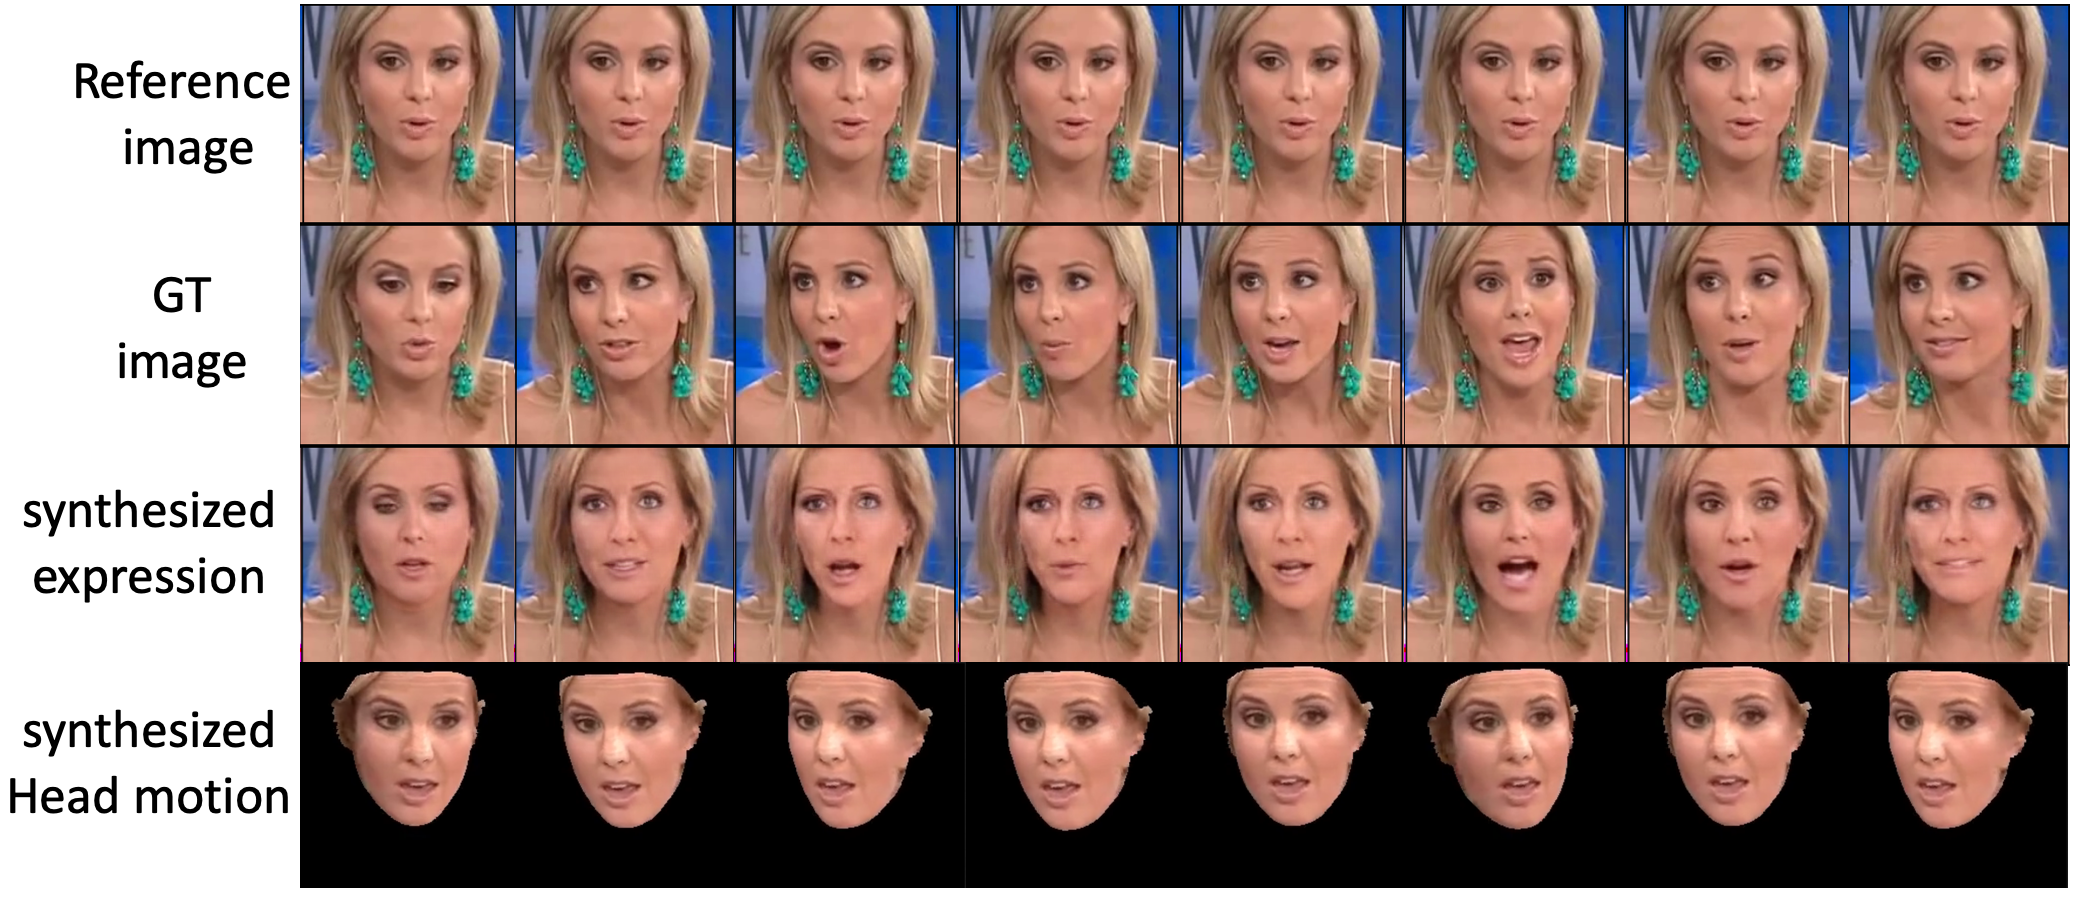
\includegraphics[width= \linewidth]{latex/images/teaser.png}
\caption{The illustration of Deepfake methods~\cite{suwajanakorn2017synthesizing,fried2019text} and our method. The green arrow denotes input. The deepfake methods require whole original video frames as input and only edit a small region (e.g., lip region) on top of the original video frames. Our method learns the appearance embedding from $K$ reference frames and learns future head movements from a 3 secs head motion vector, and can generate whole future video frames (including background) with new and controllable head movements and facial expressions.}
% \vspace{-6.5mm}
\label{fig:teaser}
\end{figure}

%PROBLEMS and some related works
We humans can infer the visual prosody from a short conversation with the speaker~\cite{munhall2004visual}. Drawing inspiration from the human perception, in this paper, we consider such a task: given a short video (e.g., 3 seconds) of the target subject and an arbitrary reference speech audio recording or reference video from a different subject, learning the individual head motion from the 3-second video and generating a photo-realistic talking-head video of the target subject that conveys the conditioned audio. The synthesized subject should have natural lip synchronization and smooth transition while moving the head with natural and rhythmic head motion. Similar problems (e.g.,~\cite{chung2017you,zhou2019talking,ijcai2019-129,vougioukas2019realistic,chen2019hierarchical,wiles2018x2face,zakharov2019few,wang2018fewshotvid2vid}) have been explored recently. However, several challenges on how to explicitly use the given video and model the large head motion remain unsolved. And we discuss our technical contributions concerning each challenge.

%CHALLENGES

%challenge 1: convoluted features.
The deformation of talking-head consists of his/her intrinsic subject traits, head movements and facial expressions, which are highly convoluted. This complexity stems not only from modeling face regions, but also from modeling head motion and background. while the synthesized talking-face conveys the input audio signal, previous audio-driven generation methods~\cite{Chung18b,wiles2018x2face,zhou2019talking,chen2018lip,ijcai2019-129,chen2019hierarchical} omit the head motion modeling thus can only generate still talking-face with expressions under a fixed facial alignment. Other landmark/image-driven generation methods~\cite{zakharov2019few,wang2018fewshotvid2vid,wang2018vid2vid,wang2018high,wiles2018x2face} are able to synthesize moving-head videos by replying on input facial landmarks or RGB video frames as the guidance to infer the convoluted head motion and facial expressions, but fail to output a controllable talking-head video (e.g., control facial expression with speech audio signal), which we argue greatly limits their use. To address the convoluted deformation problem, we propose a simple but effective method to decompose the identity appearance, head motion, and facial expression and generate controllable talking-head videos conditioned upon audio signal.     

%challenge 2: 3 seconds video.
Another challenge is exploiting the information contained in reference images/video. While the few-shot generation methods~\cite{zakharov2019few,wang2018fewshotvid2vid,liu2019few,yoo2019coloring} learn to synthesize high-quality videos of unseen subjects by leveraging $K$ reference images, they only utilize the global appearance information. There is much valuable information other than appearance. For example, we can infer the individual characteristics in head movement by leveraging the given short video. Thus, we propose a novel method to extrapolate rhythmic head motion based on the input short video while preserving a few characteristics of the individual head motion. This extrapolated head motion can be used in speech-driven talking head generation task as the head motion guidance. Furthermore, We propose a novel hybrid-attention network to dynamically aggregate features from reference images Furthermore, and a matching scheme to utilize the given video to smooth the facial movement transition and stabilize the backgrounds.

%challenge 3: 3D 
People are sensitive to any subtle artifacts and perceptual identity changes in a synthesized video, which is hard to avoid in GAN-based methods. 3D graphics modeling has been introduced by~\cite{fried2019text,kim2018deep} in GAN-based methods due to its stability. In this paper, we employ the 3D modeling along with a novel none-linear composition module to alleviate the visual discontinuities caused by large head motion, facial expressions or the overfitting problem. 

%summary
Combining above features, which are designed to overcome limitations of existing methods, our framework can generate talking-head video with natural head motion that conveys the given input condition. We conduct extensive experimental validation with comparisons to various state-of-the-art methods on several benchmark datasets (e.g., VoxCeleb2~\cite{Chung18b}, LRW~\cite{Chung16}, and VoxCeleb1~\cite{Nagrani17} datasets ) under several different settings (e.g., audio to video, landmark to video, and few-shot learning). Experimental results show that the proposed framework effectively addresses the limitations of existing talking-head generation methods.

\section{Related Work}
\label{sec:related}
In this section, we first briefly survey related work on the talking-face/head generation task. Then we discuss the related work of each technique used in our model.

\subsection{Talking-face/head Image Generation}
\label{subsec:talking-syn}
The success of graphics-based approaches has been mainly limited to synthesizing talking-head videos for a specific person~\cite{garrido2015vdub,bregler1997video,chang2005transferable,liu2011realistic,suwajanakorn2017synthesizing}. For instance, Suwajanakorn et al.~\cite{suwajanakorn2017synthesizing} produce photo-realistic videos by composite the generated lip region with existing image frame. While it can synthesize fairly accurate lip-synced videos, it requires a large amount of video footage of the target person to compose the final video. Moreover, this method can not be generalized to an unseen person due to the rigid matching scheme. More recently, video-to-video translation has been shown to be able to generate arbitrary faces from arbitrary input data. While the synthesized video conveys the input speech signal, the talking-face generation methods~\cite{chung2017you,zhou2019talking,ijcai2019-129,Vougioukas2019,chen2019hierarchical} can only generate facial expressions without any head movements under a fixed alignment since the head motion modeling has been omitted. Talking-head methods~\cite{zakharov2019few,chen2019hierarchical,wiles2018x2face} are able to generate high-quality videos with convoluted facial expression and head motion. However, due to the lack of explicit head motion modeling, these methods can not generate controllable video, e.g., using audio to drive the generation. 

\subsection{Related Techniques }
\label{subsec:related_tec}
\noindent \textbf{Head Motion Modeling} \quad
In real-world scenarios, people nautically emit head movements when we speak, which are highly convoluted with our facial expressions. Previous talking-head generation methods either omit the head motion~\cite{pumarola2019ganimation,chen2019hierarchical,chung2017you,ijcai2019-129,zhou2019talking,vougioukas2019realistic}, reply on image/landmark as dense/sparse guidance~\cite{wiles2018x2face,zakharov2019few,wang2018fewshotvid2vid}, or require a large video corpus of the target person and only edit small regions (e.g. lip regions) of the face~\cite{suwajanakorn2017synthesizing,fried2019text}. Those methods either fail to output a controllable talking-head video, or are not generalizable to unseen identities, which we argue greatly limits their use. For example, Wiles et al.~\cite{wiles2018x2face} create a dense mapping between the image paired with target pose and a embedded face of reference subject, then sample the pixels from the embedded face using the estimated mapping. This method can only generate image with target head pose and facial expression provided by the reference image, which can not be manipulated separately (e.g., drive the facial expression with audio). Some works~\cite{suwajanakorn2017synthesizing,fried2019text} generate a small region (e.g., lip region) and compose it with a retrieved frame from a large video corpus of the target person. For instance, Fried et al.~\cite{fried2019text} explore generating images with different head poses, but their method can only retrieve poses that exist in their footage database, which limits their method as a video editing method instead of a video generating method. We explicitly model the head motion and facial expression in a disentangle manner and propose a method to extrapolate rhythmic head motion for future frames to enable audio-driven talking-head generation.  

\noindent \textbf{Attention Mechanism} \quad Attention mechanism, proposed by Vondrick et al.~\cite{vondrick2016generating}, has been well explored in image/video generation task~\cite{vondrick2016generating,wang2018vid2vid,pumarola2019ganimation,chen2019hierarchical}. For instance, Pumarola et al.~\cite{pumarola2019ganimation} compute the final output image by $\hat{\mathbf{I}} = (1 - \mathbf{A}) * \mathbf{C} + \mathbf{A} * \mathbf{I}_r $, where $\mathbf{I}_r$, $\mathbf{A}$ and $\mathbf{C}$ are input reference image, attention map and color mask, respectively. The attention map $\mathbf{A}$ indicates to what extend each pixel of $\mathbf{C}$ contributes to the output image $\hat{\mathbf{I}}$. However, this attention mechanism is not working if there exits large deformation between reference frame $\mathbf{I}_r$ and target frame $\hat{\mathbf{I}}$. Wang et al.~\cite{wang2018high} use estimated optic flow to warp the $\mathbf{I}_r$ to align with $\hat{\mathbf{I}}$, which is computationally expensive and can not estimate the rotations in talking-head videos. In this paper, we propose a 3D manipulation solution along with a none-linear composition module to better tackle the misalignment problem caused by large head motion. 

\begin{figure}[t]
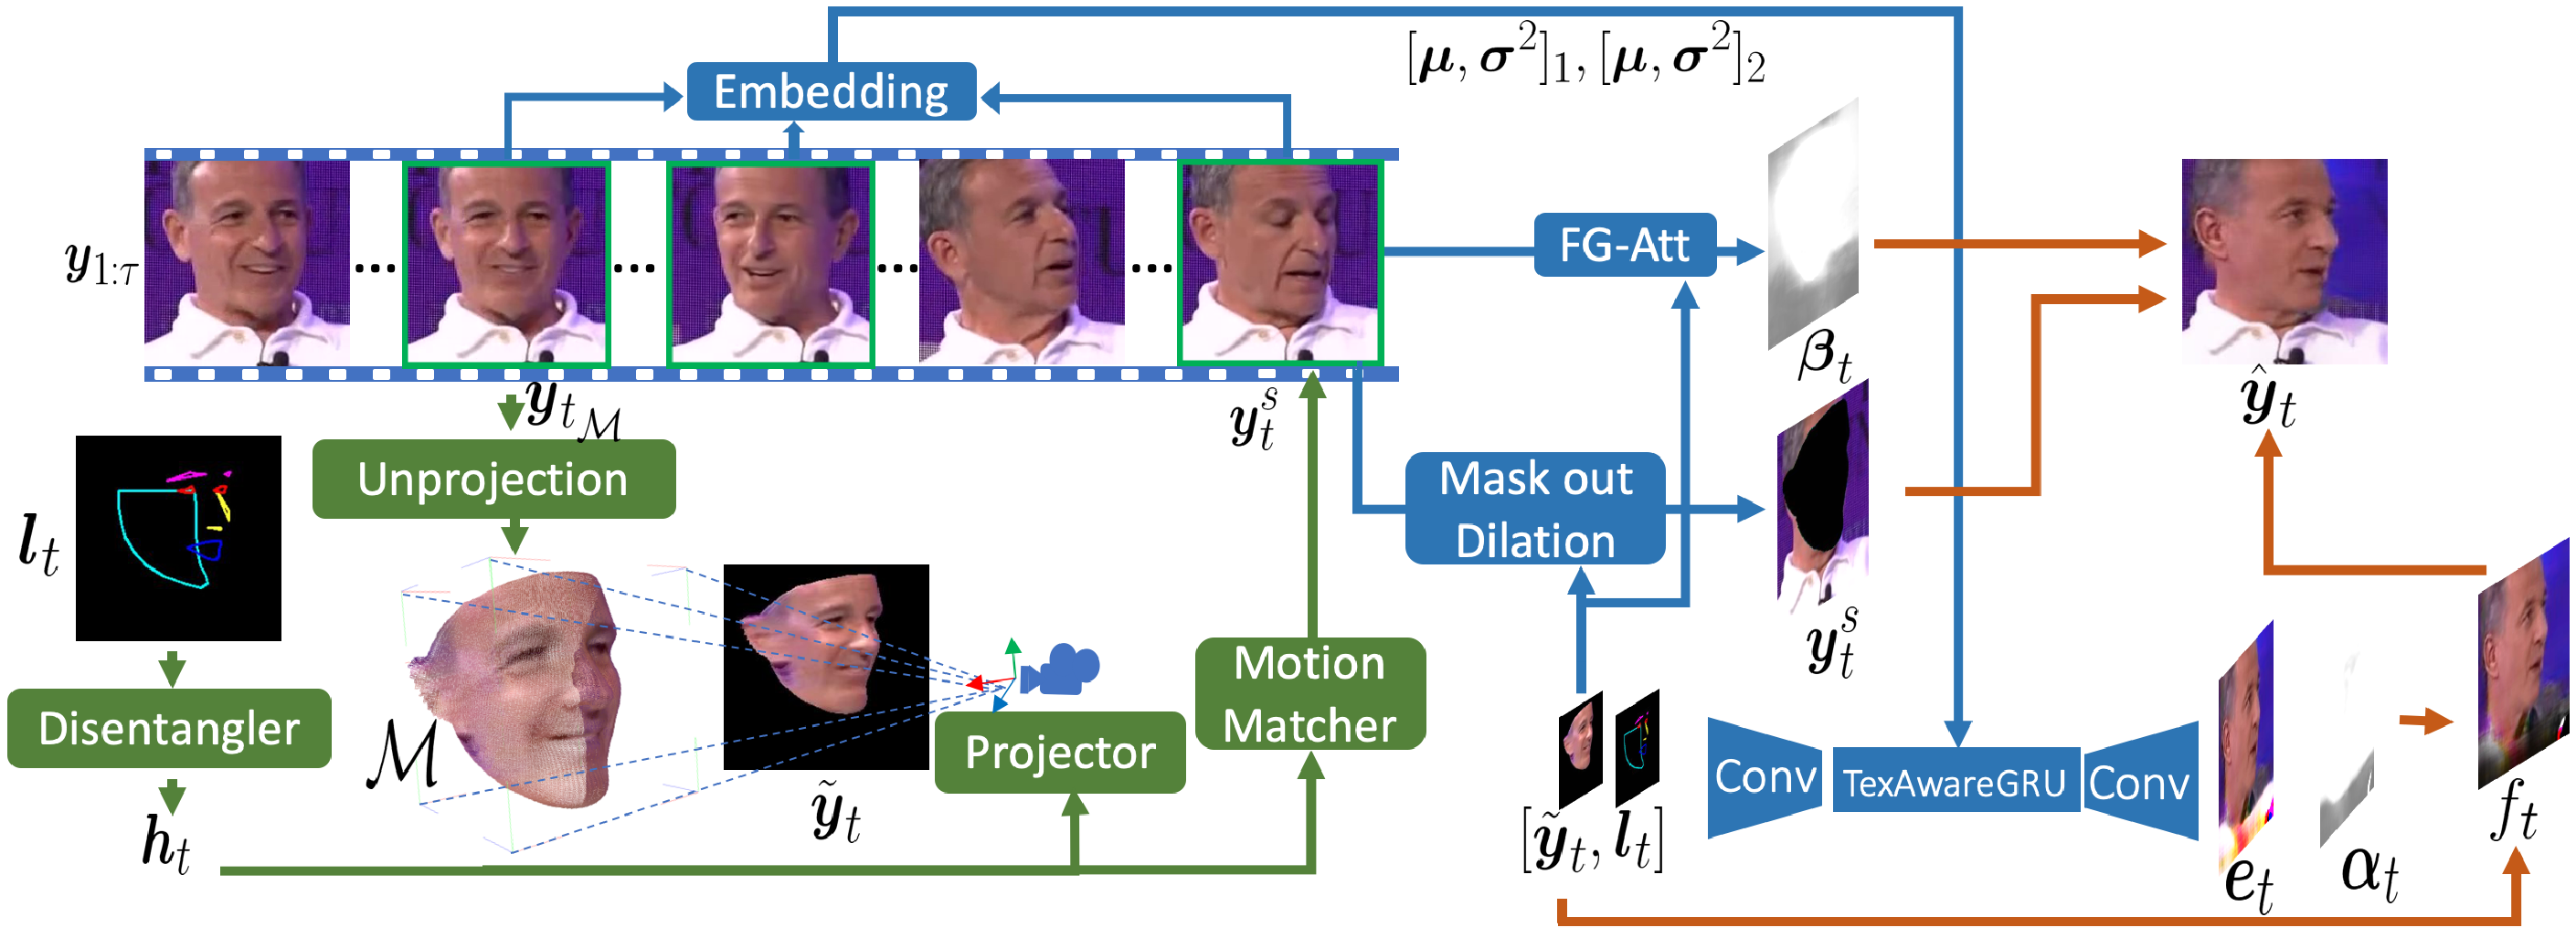
\includegraphics[width=1.0 \linewidth]{latex/images/main.pdf}
\caption{The overview of the framework.}
% \vspace{-6.5mm}
\label{fig:main}
\end{figure}

\section{Method}
\label{sec:method}

\subsection{Problem Formulation}
\label{subsec:problem_formulation}
% Hybrid-Attention for embedding network
% None-linear composition module
We introduce a neural approach for talking-head video generation leveraging temporal modeling and 3D manipulation. Our approach takes as input sampled video frames, $\mathbi{\mathbi{y}}_{1:\tau} \equiv \mathbi{\mathbi{y}}_1,...,\mathbi{\mathbi{y}}_{\tau}$, of the target subject and a sequence of driving audio, $\mathbi{\mathbi{x}}_{\tau+ 1:T}  \equiv \mathbi{\mathbi{x}}_{\tau + 1},...,\mathbi{\mathbi{x}}_T$, and synthesizes target video frames, $\hat{\mathbi{y}}_{\tau + 1:T}  \equiv \hat{\mathbi{y}}_{\tau + 1}, ...,\hat{\mathbi{y}}_T$, that convey the given audio signal with realistic head movements. To explicitly model the facial expression and head movements, we decouple the full model into three sub-models: a facial expression learner ($\Psi$), a head motion learner ($\Phi$) and a sequential generative network ($\Theta$). Specifically, given the input audio sequence $\mathbi{\mathbi{x}}_{\tau+ 1:T}$ and one example image frame $\mathbi{\mathbi{y}}_{1}$, $\Psi$ generates the facial expression $\hat{\mathbi{e}}_{\tau+1: T}$. Given the short reference video $\mathbi{\mathbi{y}}_{1:\tau}$ and audio, the $\psi$ extrapolates realistic head motion $\hat{\mathbi{h}}_{\tau + 1:T}$ to manipulate the head movements. And finally the $\Theta$ generates video frames $\hat{\mathbi{y}}_{\tau + 1:T}$ using $\hat{\mathbi{e}}_{\tau+1: T}, \hat{\mathbi{h}}_{\tau+1: T}$ and $\mathbi{\mathbi{y}}_{1:\tau}$.  Thus, the sequential generative model is given by:
\begin{equation}
\begin{aligned}
\hat{\mathbi{y}}_{ \tau+1:T} =  \Theta( \mathbi{y}_{1:\tau},\Psi( \mathbi{y}_{1} , \mathbi{x}_{\tau +1:T} ), \Phi(\mathbi{y}_{1:\tau},\mathbi{x}_{\tau +1:T} )  )  \enspace.
\end{aligned}
\label{eq:training}    
\end{equation}

The proposed framework (see Fig.~\ref{fig:main}) aims to exploit the facial texture and head motion information in $\mathbi{y}_{1:\tau}$, and maps the driving audio signal, to a sequence of generated video frames, $\hat{\mathbi{y}}_{ \tau+1:T}$. The three learners ($\Psi, \Phi, \Theta$) are trained in a decoupled way so that $\Theta$ can be trained with teacher forcing strategy. 
%We discuss the network architecture and training details of $\Psi$, $\Phi$ in Sec.~\ref{subsec:facial_exp} and Sec.~\ref{subsec:head_mo}, respectively. We briefly introduce the video generation network $\Theta$ in Sec.~\ref{subsec:3dgenerator} and extend the details is in Sec.~\ref{sec:3dgan}.
%%%%%%%%%%%%%%%%%%%%%%%%%%%%%%%%%%%%%%%%%%%%%%%%%%%%%%%%%%%%%%%%%%%%%%%%%%%%%%%%%
% key novelty 1 : 3D-Aware Head movement solver
\subsection{Facial Expression Learner}
\label{subsec:facial_exp}
The facial expression learner $\Psi$ (see Fig.~\ref{fig:main} red block) receives as input the raw audio signal $\mathbi{x}_{\tau +1:T}$, and a subject-specific RGB image $\mathbi{y}_{t_{\mathcal{M}}}$ (see Sec.~\ref{subsec:3d_man} about how to select $\mathbi{y}_{t_{\mathcal{M}}}$), from which we extract the landmark identity feature $\mathbi{p}_{t_{\mathcal{M}}}$. The desired outputs are PCA components ${\hat{\mathbi{p}}}_{\tau + 1 :T}$ that convey the facial expression. During training, we mix $\mathbi{x}_{\tau +1:T}$ with a randomly selected noise file in 6 to 30 dB SNRs with 3 dB increments to increase the network robustness. At time step $t$, $\Psi$ encodes audio clip $\mathbi{x}_{t-3:t+4}$ ($0.04 \times 7$ Sec) into audio feature, then injects the encoded reference landmark feature to it and decodes the fused feature into PCA components of target expression ${\hat{\mathbi{p}}}_{t}$. We calculate the MSE loss on the PCA components. During inference, we can add the identity feature $\mathbi{p}_{t_{\mathcal{M}}}$ back to the resultant facial expression ${\hat{\mathbi{p}}}_{t}$ to keep the identity information. 
\begin{figure}[t]
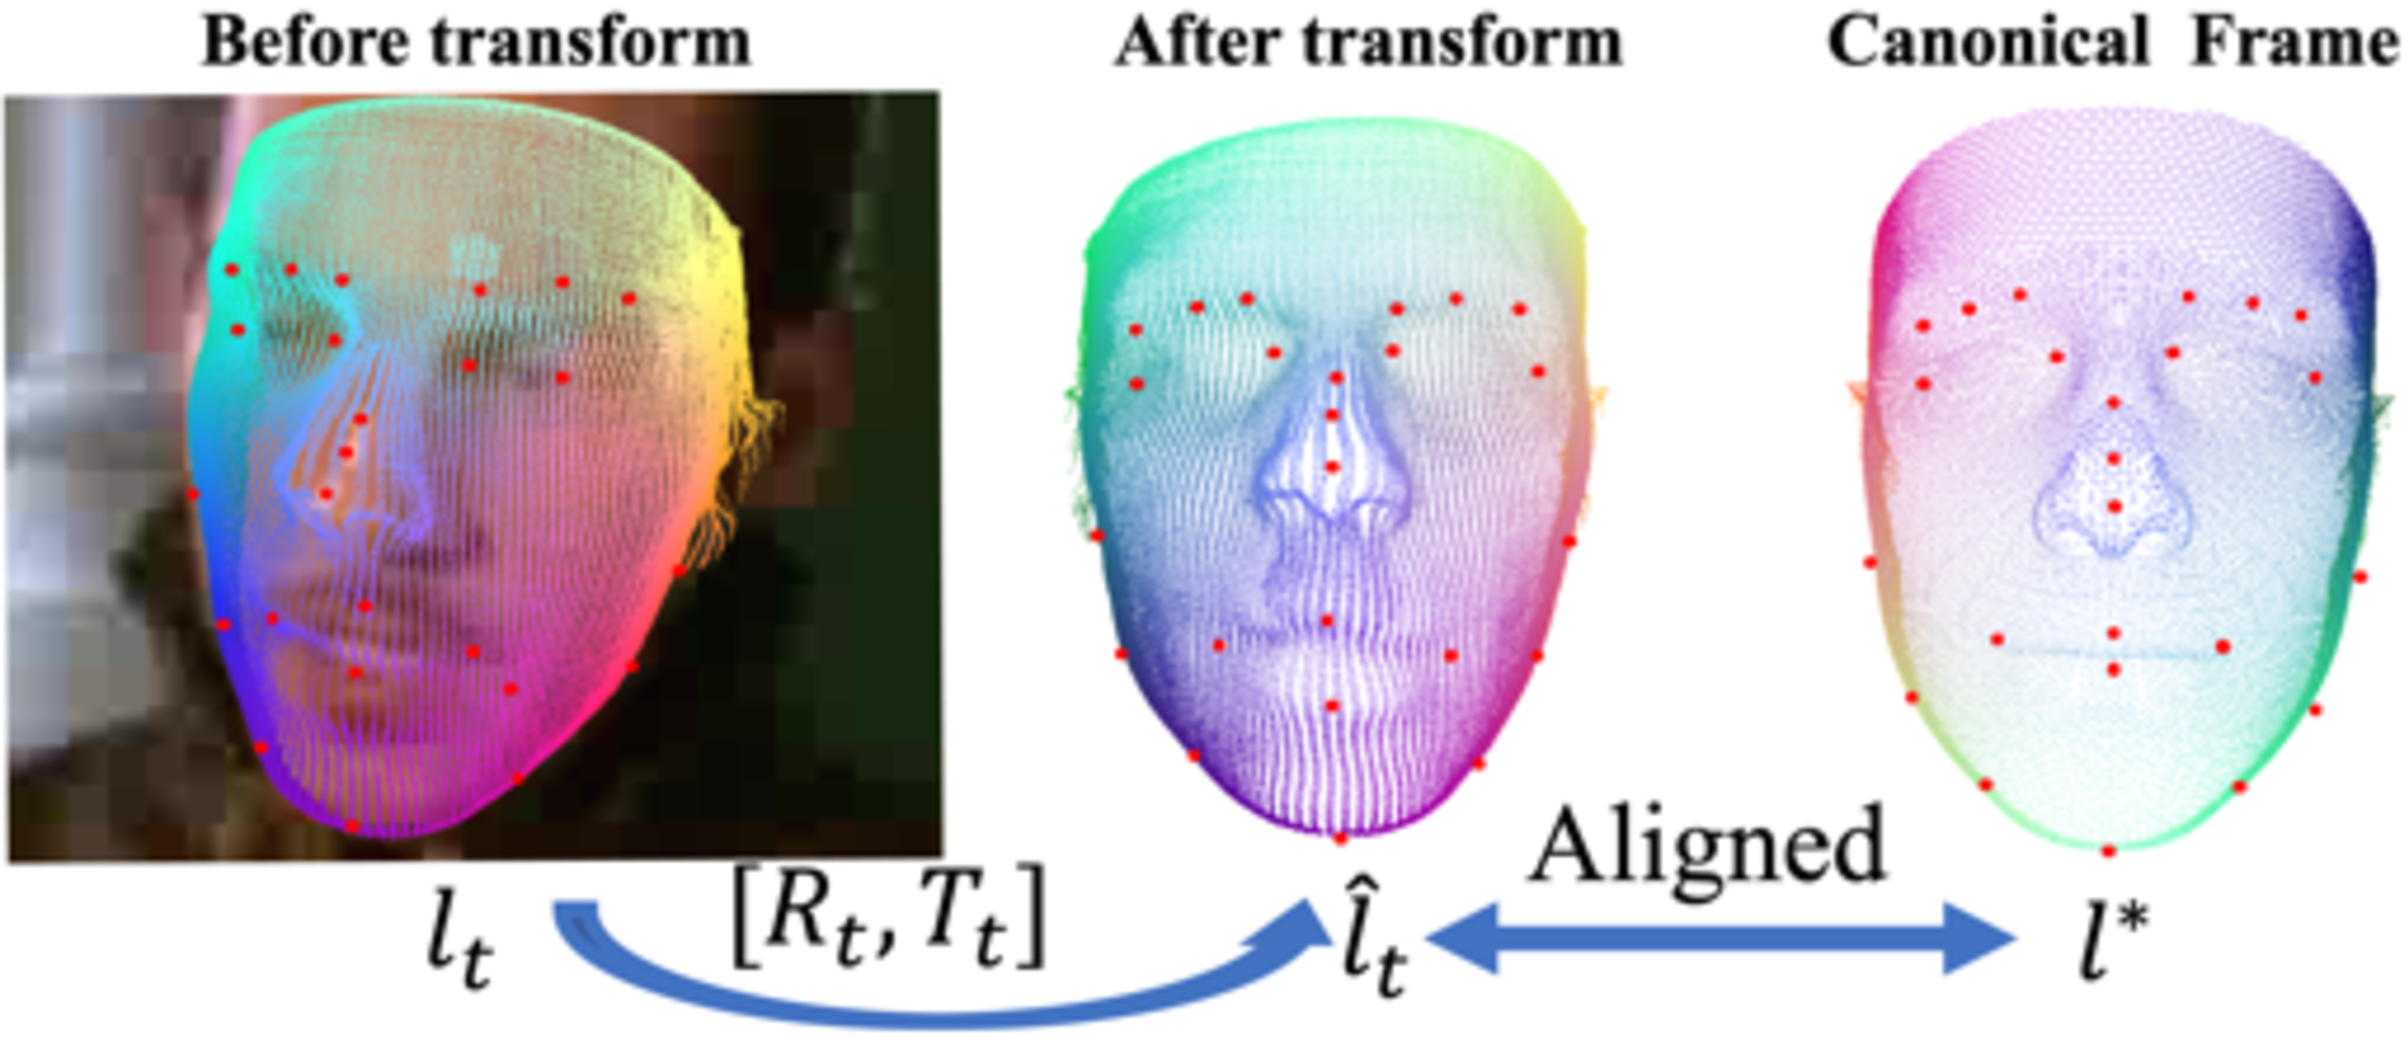
\includegraphics[width= \linewidth]{latex/images/RT_reduce.pdf}
\caption{ (a) shows the movement vector extraction. The $\mathbi{l}_t$ is the original landmark at time step t, after disentangling, the resultant $\mathbi{p}_t$ is facial expression and the estimated $[\mathbi{R,T}]_t$ is the head motion. (b) shows the head movement coefficients of randomly-selected two identities in different videos. PID, VID indicates identity id and video id, respectively. }
%The right side figure shows how to apply the computed $[\mathbf{R},\mathbf{T}]_t$ to $\mathbi{l}_t$ to get frontalized landmark $\hat{\mathbi{l}}_t$.}
% \vspace{-6.5mm}
\label{fig:rt_compute}
\end{figure}

\subsection{Head Motion Learner}
\label{subsec:head_mo}
To generate talking-head video with natural head movements, we introduce a head motion learner $\Phi$, which disentangles the reference head motion ${\mathbi{h}}_{1:\tau}$ from the input reference video clip $\mathbi{y}_{1:\tau}$, and predicts the head movements $\hat{\mathbi{h}}_{\tau +1:T}$ based on the driving audio ${\mathbi{x}}_{1:T}$ and ${\mathbi{h}}_{1:\tau}$.

 \noindent {\bf{Motion Disentangler.}}\indent Rather than disentangling the head motion problem in image space, we learn the head movements $\mathbi{h}$ in \lchen{3D geometry space}. Specifically, we compute the transformation matrix $[\mathbf{R},\mathbf{T}] \in \mathbb{R}^{6}$ to represent $\mathbi{h}$, where we omit the camera motion and other factors (see Fig.~\ref{fig:rt_compute}(a)). At each time step $t$, we compute the rigid transformation $[\mathbf{R},\mathbf{T}]_t$ from the paired face landmark $\mathbi{l}_t$ to the canonical 3D facial landmark $\mathbi{l}^*$, which is ${\mathbi{p}}_t = \mathbf{R}_t  \mathbi{l}_t + \mathbf{T}_t$. After transformation, the head movement information is removed, and the resultant ${\mathbi{p}}_t$ only carries the facial expression information, which is correlated with the input condition $\mathbi{x}_t$. To avoid the noise caused by non-rigid deformation, we select 27 points (marked as red points in Fig.~\ref{fig:rt_compute}(a)), which contain less non-rigid deformation.
 
 \noindent {\bf{The natural head motion extrapolation.}}\indent We randomly select two identities (each with four videos) from VoxCeleb2~\cite{Chung18b} and plot the motion coefficients (see Fig.~\ref{fig:rt_compute}(b)). We can observe that the same identity (same PID, different VID) has similar head motion patterns in different videos, and different identities (different PID) have different head motion patterns. To explicitly learn learning the individual's movements from ${\mathbi{h}}_{1:\tau}$ and audio-correlated head movements from ${{\mathbi{x}}}_{1:T}$, we propose a few shot temporal convolution network $\Phi$, which can be formulated as: ${\hat{\mathbi{h}}}_{\tau+1:T} = \Phi( f({{\mathbi{h}}}_{1:\tau}, {{\mathbi{x}}}_{1:\tau}), {{\mathbi{x}}}_{\tau:T})$. In details, the encoder module $f$ first encodes ${\mathbi{h}}_{1:\tau}$ and ${{\mathbi{x}}}_{1:\tau}$ to a high-dimensional feature for each individual sample, and then transforms the feature to weights for the following linear layer. The audio features are also encoded with temporal convolution blocks and then processed by the sample specific linear layer to generate ${\hat{\mathbi{h}}}_{\tau+1:T}$.
 
 %Thanks to the Lie Group framework for affine interpolation~\cite{bansal2019affine}, from two given affine transformations $\mathbb{T}_1$ and $\mathbb{T}_2$, an intermediate transformation can be represented as a $\mathbb{T}(\xi), \xi\in[0,1]$, such that $\mathbb{T}(0)=\mathbb{T}_1$ and $\mathbb{T}(1)=\mathbb{T}_2$. Specifically, for rigid transformation, the Lie group representation of the interpolated transformation between $[\mathbf{R},\mathbf{T}]_1$ and $[\mathbf{R},\mathbf{T}]_\tau$ at $\xi$, is given by:
%\begin{equation}
% \label{eqn:rtextra}
% [\mathbf{R},\mathbf{T}](\xi) = [\mathbf{R},\mathbf{T}]_1 \exp\left(\xi \log\left([\mathbf{R},\mathbf{T}]_1^{-1}[\mathbf{R},\mathbf{T}]_\tau\right)\right).
% \end{equation}
%Closed-form expressions of the exponential and log maps can be found in~\cite{bansal2019affine}.
%Therefore, $[\mathbf{R},\mathbf{T}]_{1:\tau}$ can be mapped to the parameter space $\xi_{1:\tau}=\{\xi_1,\xi_2,...,\xi_\tau\}$, such that $[\mathbf{R},\mathbf{T}](\xi_i)\approx [\mathbf{R},\mathbf{T}]_i$. Note that $\xi_1=0$, $\xi_\tau=1$ and $\xi_i (1<i<\tau)$ can be obtained by solving 
%$\underset{x}{\text{argmin}} \begin{Vmatrix}[\mathbf{R},\mathbf{T}](\xi_i) - [\mathbf{R},\mathbf{T}]_i\end{Vmatrix}_F$.
%We observed that the movement of a talking-head is bounded and has some periodic trend. Hence, we apply the Discrete Fourier Transformation on $\xi_i^\tau$ and choose the first $45$ harmonics to construct the Fourier series $\mathcal{F}(\cdot)$, such that $\mathcal{F}(i)\approx \xi_i, i\in[1,\tau]$. Then we can extrapolate $\xi_{\tau+1:T}$ by $\{\mathcal{F}(\tau+1),...,\mathcal{F}(T)\}$. Finally, applying  Eq.~\ref{eqn:rtextra} on $\xi_{\tau+1:T}$ will result to $[\hat{\mathbf{R}},\hat{\mathbf{T}]}_{\tau + 1:T}$.
%In Fig.~\ref{fig:rtextra}, we visualize the head motion by applying $[\mathbf{R},\mathbf{T}]_i$ to the reconstructed 3D face $\mathcal{M}$ and then rendering with the 3D Projector (see Sec.~\ref{subsec:3d_man}). The bottom curve in Fig.~\ref{fig:rtextra} is the parameter $\xi$ over time.
\subsection{3D Aware Generative Network}
\label{subsec:3dgenerator}
As mentioned before, landmark/image guided methods can not generate controllable videos since the head motion and facial expression are highly convoluted in RGB videos. To generate controllable videos. We propose a 3D aware generative network $\Theta$, which fuses the movement ($\hat{\mathbi{h}}_{\tau + 1:T}$), and expression ($\hat{\mathbi{p}}_{\tau + 1:T}$) with the appearance feature from ${\mathbi{y}}_{1:\tau }$ to synthesizes target video frames, $\hat{\mathbi{y}}_{\tau + 1:T}$ in a sequential 3D-aware manual. We manipulate the head motion to reconstruct an intermediate image that carries desired head pose using a differentiable unprojection-projection step to ease the burden of the generation. Comparing to landmark-only input~\cite{zakharov2019few,wang2018fewshotvid2vid,wang2018high}, it can alleviate the overfitting problem and make training converge faster. Different reference images carries different appearance information. The texture-preserving embedding module (Fig.~\ref{fig:main} blue part) is proposed to explicitly embed texture feature from different  appearance patterns by a hybrid-attention network. The none-linear composition module is proposed to stabilize the background and better preserve the individual appearance at the end of the generation while considering the temporal-dependency modeling. Comparing to other state-of-the-art face generation methods~\cite{chung2017you,pumarola2019ganimation,zhou2019talking,zakharov2019few,wang2018high}, our none-linear composition module can synthesize videos with natural lip synchronization, smoother transition and more stable background.

\section{3D-Aware Generation}
\label{sec:3dgan}
\subsection{\textit{\textbf{3D Aware}} Module}
\label{subsec:3d_man}
%\ytian{whether it is better to add one sentence to describe input/output and the goal of the module?}
% We introduce the \textit{3D Aware} Module in the following three components: 

{ \noindent {\bf{3D Unprojection}}\indent Here, we assume that the image with frontal face contains more appearance information. Given a short reference video sequence $\mathbi{y}_{1:\tau}$, we compute the head rotation $\mathbf{R}_{1:\tau}$ and choose the most visible frame $\mathbi{y}_{t_{\mathcal{M}}}$ with minimum rotation such that $\mathbf{R}_{t_{\mathcal{M}}} \rightarrow 0$. Then we feed it to an unprojection network to unproject it to 3D mesh $\mathcal{M}$. The Unprojection network is a U-net structure network~\cite{feng2018joint} and we pretrain it on  300W-LP~\cite{zhu2016face} dataset to transfer the input RGB image into position map image. After pretrianing, we fix the weight and use it to transfer the input image $\mathbi{y}_{t_{\mathcal{M}}}$ into 3D mesh $\mathcal{M}$.}
 
\noindent {\bf{3D Projector}}\indent  In order to get the projected $\tilde{\mathbi{y}}_t$ from the 3D face mesh $\mathcal{M}$, we need to compute the correct pose for $\mathcal{M}$ at time $t$. Suppose $\mathcal{M}$ is reconstructed from frame $\mathbi{y}_{t_{\mathcal{M}}}, (1\le t_{\mathcal{M}}\le \tau)$. Then the position of vertices of $\mathcal{M}$ at time step $t$ can be computed by
\begin{equation}
\begin{aligned}
\mathcal{V}^{\mathcal{M}}_t = \mathbf{R}_t^{-1}(\mathbf{R}_{t_{\mathcal{M}}}\mathcal{V}^{\mathcal{M}}_{t_{\mathcal{M}}} + \mathbf{T}_{t_{\mathcal{M}}} - \mathbf{T}_t) \enspace.
\end{aligned}
\label{eq:projector}    
\end{equation}
The topology of $\mathcal{M}$ will be fixed for all frames in one video, we denote it as $\mathcal{F}^{\mathcal{M}}$. Hence, $\mathcal{M}$ at $t$ can be represented as $\left[\mathcal{V}^{\mathcal{M}}_t, \mathcal{F}^{\mathcal{M}}\right]$. Finally, a differentiable rasterizer~\cite{liu2019softras} is applied here to render $\tilde{\mathbi{y}}_t$ from $\left[\mathcal{V}^{\mathcal{M}}_t, \mathcal{F}^{\mathcal{M}}\right]$. After rendering, $\tilde{\mathbi{y}}_t$ carries the same head pose from target frame ${\mathbi{y}}_{t}$ and the same expression from  ${\mathbi{y}}_{t_{\mathcal{M}}}$. So, the landmark of the projected frame can be obtained by $\tilde{\mathbi{l}}_t= \mathbi{h}_t \circledast \mathbi{p}_{t_{\mathcal{M}} }$, where $\circledast$ denotes the inverse operator of motion disentangler in Sec.~\ref{subsec:head_mo}.

\noindent {\bf{Motion Matcher}}\indent To infer the prior knowledge about the background of the target image from the given $K$ reference video frames, we propose a motion matcher, $M(\hat{\mathbi{h}}_t, \mathbi{h}_{1:K}, \mathbi{y}_{1:K})$, which matches a frame $\mathbi{y}_t^s$ with nearest head motion from the sampled reference images $\mathbi{y}_{1:K}$ by comparing the similarities between $\mathbi{h}_{t}$ with $\mathbi{h}_{1:K}$. Specifically, given the query head motion $\hat{\mathbi{h}}_t$, we are looking for the optimal image $\mathbi{y}_t^s$ that contains the most similar background as the target image $\mathbi{y}_t$ (without knowing $\mathbi{y}_t$). To solve this background retrieving problem, rather than directly compute the similarity between facial landmarks, we compute the geometry similarity cost $c_{t}$ using the head motion $\mathbi{h}_t$ and choose the $\mathbi{y}_t^s$ with the least cost $c_t$. That is:
\begin{equation}
\begin{aligned}
c_{t}= \min_{k=1,2,...K}  \lVert \mathbi{h}_t - \mathbi{h}_k \rVert^2_2 \enspace.
\end{aligned}
\label{eq:cost}    
\end{equation}
  Then, the matched $\mathbi{y}_t^s$ will be a input to the none-linear composition module in Sec.~\ref{subsec:none-linear} since it carries the most similar background pattern to the target frame ${\mathbi{y}}_t$. During training, we manipulate the selection of $\mathbi{y}_t^s$ by increasing the cost $c_{t}$, which makes the none-linear composition module more robust to $\mathbi{y}_t^s$.  
  %Then, based on $\tilde{\mathbi{y}}_t$, we compute a binary mask, dilate it with 5 iterations and mask out the head regions in $\mathbi{y}_t^s$ using the dilated binary mask. The masked image frame $\mathbi{y}^s_{t}$ will be passed to the \textit{AttBuilder} module (see Sec.~\ref{subsec:AttBuilder}) as input. 
 %%%%%%%%%%%%%%%%%%%%%%%%%%%%%%%%%%%%%%%%%%%%%%%%%%%%%%%%%%%%%%%%%%%%%%%%%%%%%%%%%%
 \begin{figure}[t]
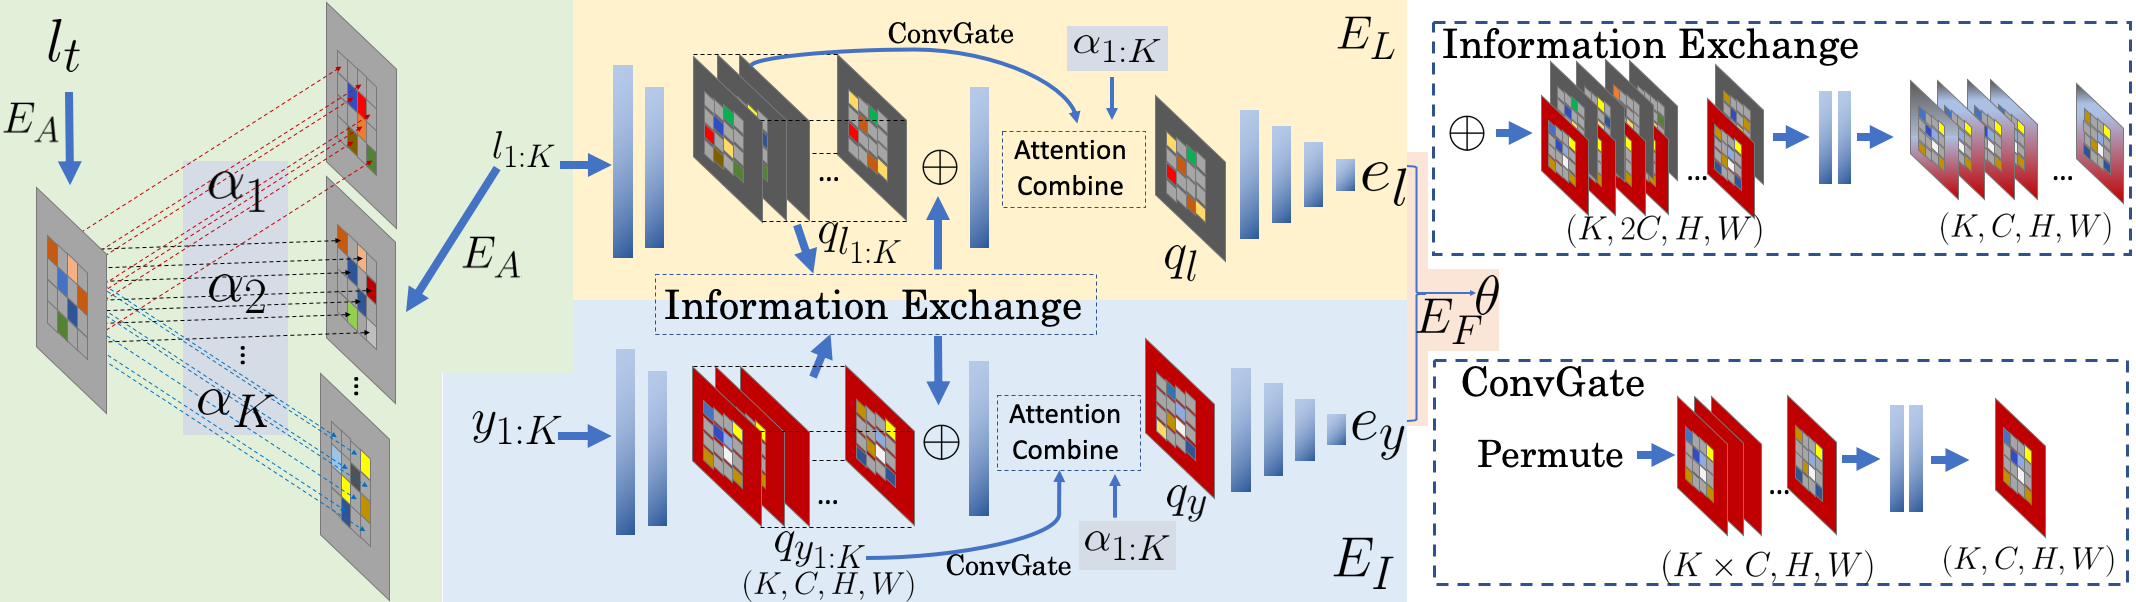
\includegraphics[width= \linewidth]{latex/images/attention.png}
\caption{The network structure.}
\label{fig:attention}
\end{figure}

\subsection{Hybrid Embedding Module}
\label{subsec:details}
We randomly select $K$ frames, $\mathbi{y}_{1:K}$ from $\mathbi{y}_{1:\tau}$ as reference images, and transfer the corresponding facial landmarks to gray-scale images $\mathbi{l}_{1:K}$. Instead of averaging the $K$ reference image features~\cite{zakharov2019few,chung2017you,wiles2018x2face}, we design a hybrid embedding mechanism to dynamically aggregate the $K$ visual features.

Fig.~\ref{fig:attention} shows the structure of our hybrid embedding network, which consists of four sub-networks: the Activation Encoder ($E_{A}$, green part) to generate the activation map between the query landmark $\mathbi{l}_t$ and reference landmarks $\mathbi{l}_{1:K}$, an Image Embedding network ($E_{I}$, blue part) to extract the image feature $\mathbi{e}_{y}$, a Landmark Embedding network ($E_{L}$, yellow part) to extract landmark feature $\mathbi{e}_{l}$, and a fusion network ($E_{F}$, pink part) to aggregate image feature and landmark feature into parameter set $\theta$. The overview of the embedding network is performed by:
\begin{align}
\label{eq:attention}
&\boldsymbol{\alpha}_{k} = \text{softmax}( E_{A}(\mathbi{l}_k) \odot E_{A}(\mathbi{l}_t))\enspace , k \in [1,K]
\enspace, \\
\label{eq:img_embed}
&\mathbi{e}_{\mathbi{y}} =  E_{I}(\mathbi{y}_{1:K}, \boldsymbol{\alpha}_{1:K})
\enspace,  \mathbi{e}_{\mathbi{l}} =  E_{L}(\mathbi{l}_{1:K}, \boldsymbol{\alpha}_{1:K})   \enspace, \\
\label{eq:fusion}
&\theta  = E_F(\mathbi{e}_{\mathbi{l}}, \mathbi{e}_{\mathbi{y}}) \enspace, 
\end{align}
% talk about the fusion network
where $\odot$ denotes element-wise multiplication. We regard the activation map $\boldsymbol{\alpha}_{k}$ as the activation energy between ${k^{th}}$ reference landmark and target landmark, which approximates the similarity between the ${k^{th}}$ reference image and the target image. 

We observed that different reference images may carry different appearance pattern, and those appearance pattern shares some features with the reference landmarks (e.g., head pose, and edges). Assuming that knowing the information of one modality can better encode the feature of another modality, we hybrid the information between $E_{I}$ and $E_{L}$. Specifically, after two convolutional layers, the extracted feature map $\mathbi{q}_{y_{1:K}}$ and $\mathbi{q}_{l_{1:K}}$ are forwarded to a information exchange block to refine their feature. Then the hybrid feature is concatenated with the original $\mathbi{q}_{y_{1:K}}$ and $\mathbi{q}_{l_{1:K}}$, and we pass the concatenated feature to a bottleneck convolution layer to produce the refined feature $\mathbi{q}^'_{y_{1:K}}$. At the meanwhile, we apply a ConvGate operation on $\mathbi{q}_{y_{1:K}}$ to self-aggregate the features from $K$ references, and then combine the gated feature and refined feature with the learnable activation map $\boldsymbol{\alpha}_{k}$:
\begin{align}
\label{eq:qy_combine}
\mathbi{q}_{y}= \sum_{i=1}^{K} (\boldsymbol{\alpha}_{1:K} \odot \mathbi{q}^'_{y_{1:K}}) + \text{ConvGate}(\mathbi{q}_{y_{1:K}})
\enspace.
\end{align}
Then, we apply several convolutional layers on the aggregated feature $\mathbi{q}_{y}$ and obtain the image feature vector $\mathbi{e}_y$. The landmark feature vector $\mathbi{e}_{l}$ is produced by following the same process.

The Fusion network $E_{F}$ consists of three blocks: a $N$-layer image feature encoding block $E_{F_{I}}$, a landmark feature encoding block $E_{F_L}$, and a multi-layer perception block $E_{F_{p}}$ to aggregate reference features into appearance parameter set $\theta$:
\begin{align}
\label{eq:fusion2}
\{\theta_\gamma^i, \theta_\beta^i, \theta_S^i\}_{i \in [1,N]} = E_{F_p}({\text{softmax}}(  E_{F_L}(\mathbi{e}_{\mathbi{l}})) \odot E_{F_I}(\mathbi{e}_{\mathbi{y}}) )
\enspace,
\end{align}
where $\{\theta_\gamma^i, \theta_\beta^i, \theta_S^i\}_{i \in [1,N]}$ is the parameters of the $N$ layers of the none-linear composition module in Sec.~\ref{subsec:none-linear}.


%The appearance latent vector $\mathbi{z}_y$ computed from the embedding network contains the global texture information of target identity. At each time step $t$, after encoding the input pair $[\mathbi{l}_t, \tilde{\mathbi{y}}_{t}]$, the resultant feature $\mathbi{e}_t$ carries the detailed facial expression and geometry information. Rather than simply concatenating the feature vectors~\cite{chung2017you,zhou2019talking,chen2018lip,chen2019hierarchical,ijcai2019-129}, we propose a \textit{TP-GRU} module, which aims to fuse appearance feature, geometry feature and expression feature in a recurrent manner. The \textit{TP-GRU} (see right part in Fig.~\ref{fig:network_details}) consists of eight convolution layers with residual connections and one layer of convolutional GRU. There are four convolution layers normalized by adaptive instance normalization (AdaIN)~\cite{huang2017arbitrary}. The AdaIN layers are initialized with zero means and unit variance at each time step. We then adaptively compute two sets of affine transformation parameters $[\boldsymbol{\mu},\boldsymbol{\sigma}^2]_1, [\boldsymbol{\mu},\boldsymbol{\sigma}^2]_2$ using $\mathbi{z}_y$ via two separately-learnable fully connected perceptions. We apply the two sets of parameters as scalars and biases to scale the activations in the two AdaIN layers before and after GRU, respectively. The intuition is that the affine transformation is spatially invariant and hence we can inject global appearance information to \textit{TP-GRU}. We empirically show TP-GRU learn to fuse novel appearance and strongly generalize to novel identities with different poses, appearances, and expressions (see Tab.~\ref{tab:lmark_tb} CSIM score).  %To avoid the error accumulation caused by $\hat{\mathbi{p}}_{\tau + 1:T}$ and $\hat{\mathbi{h}}_{\tau + 1:T}$, $\Theta$ is conditioned on ground truth facial expression ${\mathbi{p}}_{\tau + 1:T}$ and head motion ${\mathbi{h}}_{\tau + 1:T}$ during training.

\begin{figure}[t]
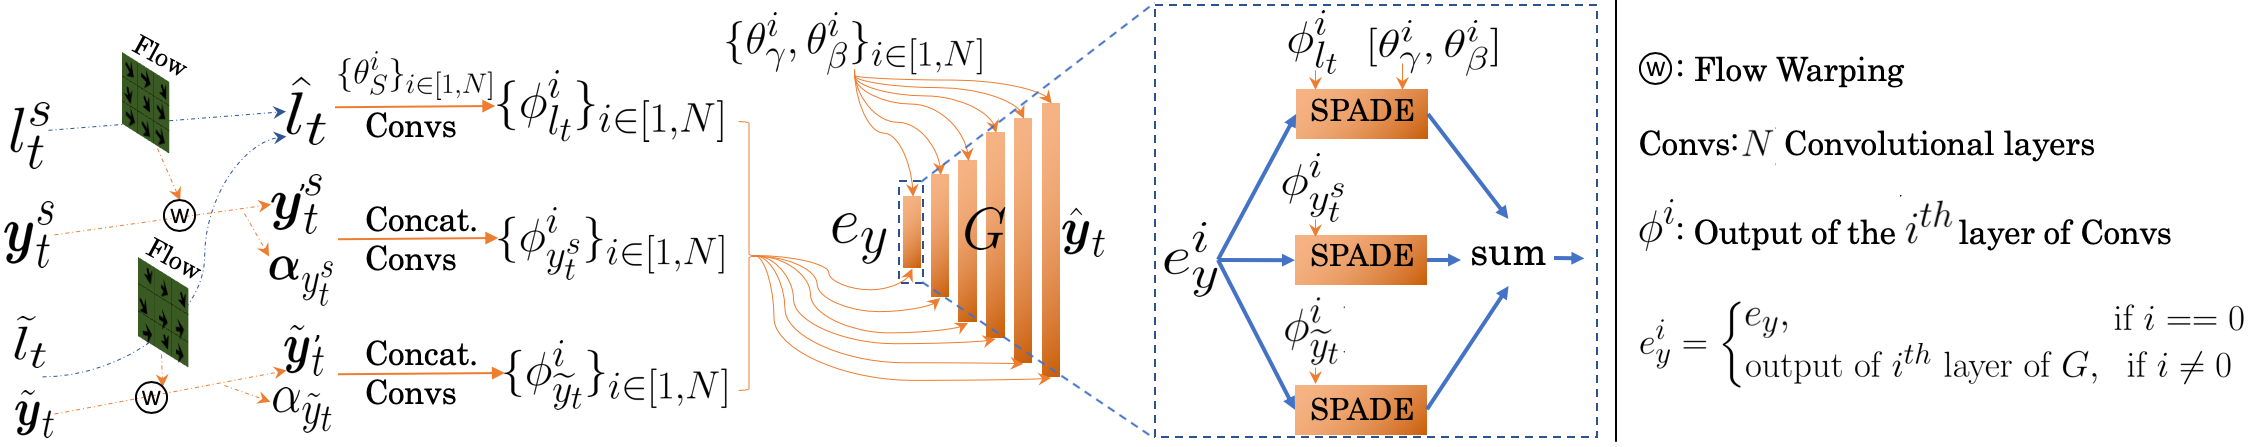
\includegraphics[width= \linewidth]{latex/images/3dgan.png}
\centering
\caption{The network structure.}
\label{fig:composite}
\end{figure}

\subsection{None-Linear Composition Module} 
\label{subsec:none-linear}
As mentioned before that the projected image $\tilde{\mathbi{y}}_t$ carries valuable texture information with better alignment to the ground-truth $ \mathbi{y}_t$, and the matched image $\mathbi{y}_t^s$ contains similar background pattern. To ease the burden of the generation, we input $\mathbi{y}_t^s$ and $\tilde{\mathbi{y}}_t$ as extra guidance to the generator $G$. Specifically, we obtain the warped image $\mathbi{y}_t^{'s}$ and $\tilde{\mathbi{y}}_t^{'} $ guided by the flow estimated between ${\mathbi{l}}^s_t, {\tilde{\mathbi{l}}}_t$ and ${\hat{\mathbi{l}}}_t$, respectively. We add one more branch at the last layer of the FlowNet~\cite{wang2018vid2vid}, which consists of one convolutional layer and a sigmoid activation, to yield the corresponding attention maps $\boldsymbol{\alpha}_{y_t^s}$ and $\boldsymbol{\alpha}_{\tilde{y}_t}$. Taking these attention maps as guidance, image matting function is a popular way to combine warped image with raw output of generator~\cite{wang2018fewshotvid2vid,wang2018vid2vid,chen2019hierarchical,pumarola2019ganimation}, but it may introduce obvious artifacts to $\hat{\mathbi{y}}_{t}$ caused by misalignment, which is amplified in the videos with large head movements. 

To solve the misalignment problem, we introduce a nonlinear combination module (see Fig.~\ref{fig:composite}). specifically, given the projection pair $[\tilde{\mathbi{y}}_t^{'},\boldsymbol{\alpha}_{\tilde{y}_t}]$, and matching pair $[\mathbi{y}_t^{'s}, \boldsymbol{\alpha}_{{y}_t^s}]$ 
 
 We embedded warped image and attention map pairs into $N$ groups of features $[E_t^{sm},\tilde{E}_t^m, \hat{E}_{t-1}^m], m\in [1, N]$ with $N$ convolutional layers, and then input them into SPADE~\cite{park2019semantic} to normalize corresponding feature maps of $e_y$ in generator $G$. Fusing warped image and $e_y$ in such high level representation results in more natural texture in $\hat{\mathbi{y}}_{t}$. Additionally, in order for better consistency between landmark $\hat{l}_t$ and $\hat{\mathbi{y}}_{t}$, we embedded $\hat{l}_t$ into $M$ features $\hat{E}_t^{lm}$ and append them together with $[E_t^{sm},\tilde{E}_t^m, \hat{E}_{t-1}^m]$ as input of SPADE. Follow~\cite{wang2018fewshotvid2vid}, $[\theta_s^n]$ are used for parameters of convolutional kernel to encode $\hat{l}_t$, and $[\theta_\gamma^n, \theta_\beta^n]$ are used for parameters of SPADE in generator to extract normalization maps.

 For further comparison to linear-combination, our method is more robust to the spatial-misalignment between the two input images, especially when there is large head motion between the input frame and the ground-truth frame. Moreover, in our empirical study, this composition can correct the identity mismatch in the generation stage and make the network converge faster.


%We build our none-linear generator module based on ~\cite{wang2018fewshotvid2vid,wang2018vid2vid,park2019semantic}, which are the state-of-the-arts for image/video generation task.
%After the \textit{TP-GRU} module, the frame feature $\mathbi{e}_t$ is up-sampled by several convolutional blocks with an up-sampling layer. Similar to~\cite{pumarola2019ganimation}, we apply convolution with sigmoid and hyperbolic tangent activation functions on the up-sampled image feature to get texture attention map $\boldsymbol{\alpha}_t \in \mathbb{R}^{H\times W \times1}$ and synchronized facial motion map $\mathbi{m}_t \in \mathbb{R}^{H\times W \times C}$, respectively. As mentioned before, our animation frame $\tilde{\mathbi{y}}_t$ also contains valuable texture information with better alignment to the ground-truth $ \mathbi{y}_t  $. Thus the foreground of the image $f_t \in \mathbb{R}^{H\times W \times C}$ at time step $t$ is governed by the combination:
%\begin{equation}
%\begin{aligned}
% f_t =   \boldsymbol{\alpha}_t \odot \mathbi{m}_t + (\mathbf{1}- \boldsymbol{\alpha}_t ) \odot \tilde{\mathbi{y}}_t  %\enspace,
%\end{aligned}
%\label{eq:foreground}    
%\end{equation}
%where the $\odot$ is element-wise multiplication. Note that compared to previous methods~\cite{pumarola2019ganimation,chen2019hierarchical,wang2018high}, which use a reference image rather than $\tilde{\mathbi{y}}_t$, our combination method is much better in talking-head video generation task especially when there is large head motion between reference frames and the ground-truth frame. Furthermore, in our empirical study, this composition can correct the identity mismatch in the generation stage and make the network converge faster. 

%We observe that the background of target image $\mathbi{y}_t$ at step $t$ is expected to be, on average, more visually similar to image that contains head with similar pose in a video recorded by still camera. The combination of foreground $f_t$ and background $\mathbi{y}_t^s$ follows the similar protocol in Eq.~\ref{eq:foreground}. We apply a Foreground-Attention (FG-Att) on $\mathbi{y}_t^s$, $ \tilde{\mathbi{y}}_t$ and the frame feature $\mathbi{e}_t$ to obtain the foreground attention. Specifically, we concatenate  $\mathbi{y}_t^s$ and $\tilde{\mathbi{y}}_t$ in channel-wise to $[\mathbi{y}_t^s, \tilde{\mathbi{y}}_t] \in \mathbb{R}^{H\times W \times 2C}$ and apply three convolutional layers on it to have a prior foreground feature $\mathbi{p}_t \in \mathbb{R}^{H\times W \times 64}$ and concatenate with the frame feature $\mathbi{e}_t$ in channel wise to have $[\mathbi{p}_t, \mathbi{e}_t] \in \mathbb{R}^{H\times W \times 128}$. Then we feed the concatenated feature to one convolution layer with sigmoid activation function to compute an adaptively learned foreground attention map $\boldsymbol{\beta}_t \in \mathbb{R}^{H\times W \times 1}$. With this foreground attention map, dilated background image $\mathbi{y}_t^s$ and computed foreground $f_t$, the final image frame is obtained by:
% \begin{equation}
% \begin{aligned}
%  \hat{y}_t =   \boldsymbol{\beta}_t \odot f_t + (\mathbf{1}- \boldsymbol{\beta}_t ) \odot\mathbi{y}_t^s  \enspace.
% \end{aligned}
% \label{eq:background}    
% \end{equation}
% We apply dilation operation on $\mathbi{y}_t^s$ to alleviate the misalignment issue caused by $c_t$ in the motion matching step. We also tried to learn an optic flow from $[f_t, \mathbi{y}_t^s ]$ to warp $\mathbi{y}_t^s$ to fix the misalignment issue, but the results show that dilation is more efficient and accurate (see Tab.~\ref{tab:alation}).
 
\subsection{Objective Function}
\label{subsec:loss}

The Multi-Scale Discriminators~\cite{wang2018high} are employed to differentiate the real and synthesized video frames. We use two discriminators that have the same network structure but operate at two different image scales. At each time step $t$, we downsample the pair of image frame and associated converted landmark image $[\mathbi{l}_{t}, \mathbi{y}_{t}] \in \mathbb{R}^{H\times W \times 2C} $ by a factor of 2 to create an pyramid of two scales. The discriminators $D_1$ and $D_2$ are trained on the two input scales, respectively. Thus, the best sequential generator $G^*$ is found by solving the following optimization problem:
\begin{equation}
\begin{aligned}
& G^* = \argminA_G\bigg{(} \Big{(} \max_{D_1,D_2}\sum_{k=1,2} \mathcal{L}_{\text{GAN}}(G,D_k) \\
& + \lambda_{\text{FM}} \sum_{k=1,2} \mathcal{L}_{\text{FM}}(G,D_k) \Big{)} + \lambda_{\text{PCT}} \mathcal{L}_{\text{PCT}}(G)\bigg{)}  \enspace,
\end{aligned}
\label{eq:loss}    
\end{equation}
where $\mathcal{L}_{\text{GAN}}$ is the LSGAN loss~\cite{mao2017least}, $\mathcal{L}_{\text{FM}}$ is the feature matching loss proposed in 
~\cite{wang2018high} to stabilize the training. The $\mathcal{L}_{\text{PCT}}$ is the perceptual loss term, which measures the perceptual similarity distance between the ground truth video frames and the synthesized video frames. The $\lambda_{\text{FM}}$ and $\lambda_{\text{PCT}}$ control the importance of three loss terms. 

The perceptual loss~\cite{johnson2016perceptual} term $\mathcal{L}_{\text{PCT}}$ in Eq.~\ref{eq:loss} regularizes the training in two different perceptual respects: we employ the VGG19~\cite{Simonyan15} feature extractor pretrained on ImageNet~\cite{deng2009imagenet} classification to increase the sharpness of synthesized video. The VGGFace~\cite{parkhi2015deep} feature extractor pretrained on the VGG-Face dataset is employed to consider the identity similarities between synthesized videos and ground truth videos.  


% \section{Talking-head Generation with rhythmic head motion }
% \label{sec:infer}

% % \CXu{This section tells about inference with different strategies, or aka driving modalities.}

% During training (see Sec.~\ref{sec:method}), we generate videos based on ground truth landmarks $\mathbi{l}_{\tau+1:T}$ in order to supervise the training. In other word, we use ground truth head motion $\mathbi{h}_{\tau+1:T}$ and ground truth facial expression $\hat{\mathbi{l}}_{\tau+1:T}$ to synthesize videos. At the inference stage, the facial expression $\hat{\mathbi{l}}_{\tau+1:T}$ can be transferred from user input data ${\mathbi{x}}_{\tau+1:T}$ (e.g., audio signal, landmarks and RGB frames). And the head movement ${\mathbi{h}}_{\tau+1:T}$ can be inferred either from conditioned videos or the 3-second video ${\mathbi{y}}_{1:\tau}$ of the target subject. Here, we mainly discuss such a novel protocol: we generate $\hat{\mathbi{l}}_{\tau+1:T}$ from an arbitrary speech signal, and infer $\hat{\mathbi{h}}_{\tau+1:T}$  from the input short video ${\mathbi{y}}_{1:\tau}$. So the Eq.~\ref{eq:training} can be rewritten as:9
% rea\begin{equation}
% \begin{aligned}
% \hat{\mathbi{y}}_{ \tau+1:T} =  F( \mathbi{y}_{1:\tau},\hat{\mathbi{l}}_{\tau+1:T}   \circledast \hat{\mathbi{h}}_{\tau+1:T} )  \enspace,
% \end{aligned}
% \label{eq:inference}    
% \end{equation}
% where the $\circledast$ is the inverse operator of motion disentangler in Sec.~\ref{subsec:3d_man} and $\hat{\mathbi{h}}_{\tau+1:T}$ can be approximated in Sec.~\ref{subsec:movement}.
% %
% %our model can generate video based on an arbitrary audio signal or an arbitrary video/landmark sequence. We transfer the input audio signal/video sequence to facial landmarks and use \textit{motion disentangler} to disentangle the facial expression $\hat{\mathbi{l}}_{\tau+1:T}$, which only contains facial-expression-correlated information. Then we use the head motion extrapolation module to extrapolate the individual head movements $\hat{\mathbi{h}}_{\tau+1:T}$ using the input reference video. Next, based on the extrapolated head motion $\hat{\mathbi{h}}_{\tau+1:T}$ and 3D mesh $\mathcal{M}$, our projector outputs corresponding 3D projection $\tilde{\mathbi{y}}_{\tau+1:T}$. Then we feed the manipulated facial landmark with corresponding 3D animation $[\hat{\mathbi{l}}_{\tau+1:T}  \circledast \hat{\mathbi{h}}_{\tau+1:T}, \tilde{\mathbi{y}}_{\tau+1:T} ] $ to the framework to get the synthesized video sequence $\hat{\mathbi{y}}_{\tau+1:T}$. 
% The facial expressions are controlled by $\hat{\mathbi{l}}_{\tau+1:T}$ and the $\hat{\mathbi{h}}_{\tau+1:T}$ carries the natural head motion. 
 
 
% \begin{figure}
% 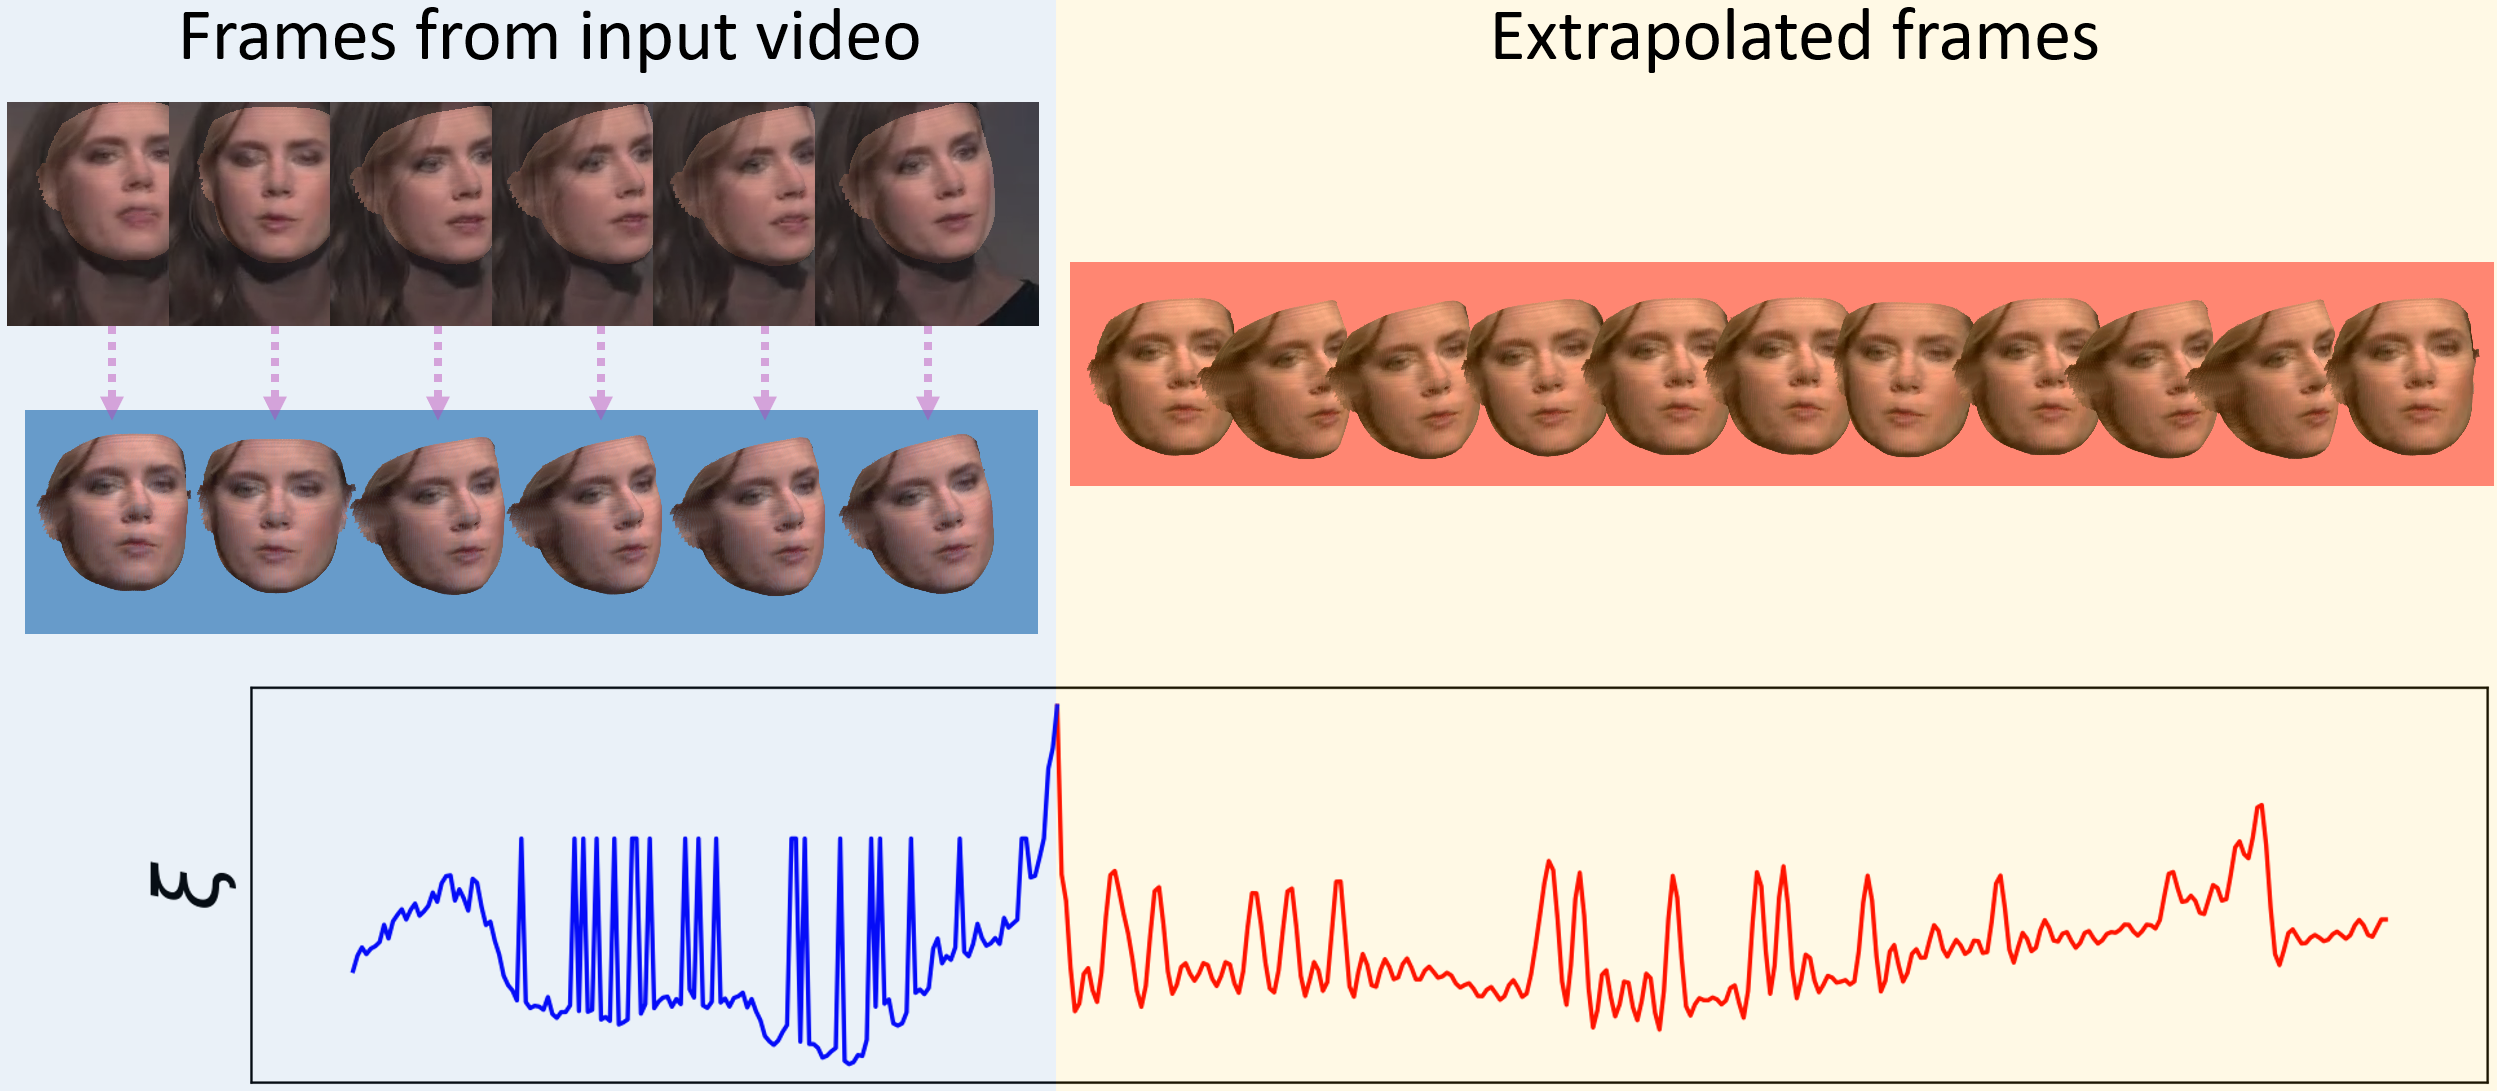
\includegraphics[width=1.0 \linewidth]{latex/images/faces.png}
% %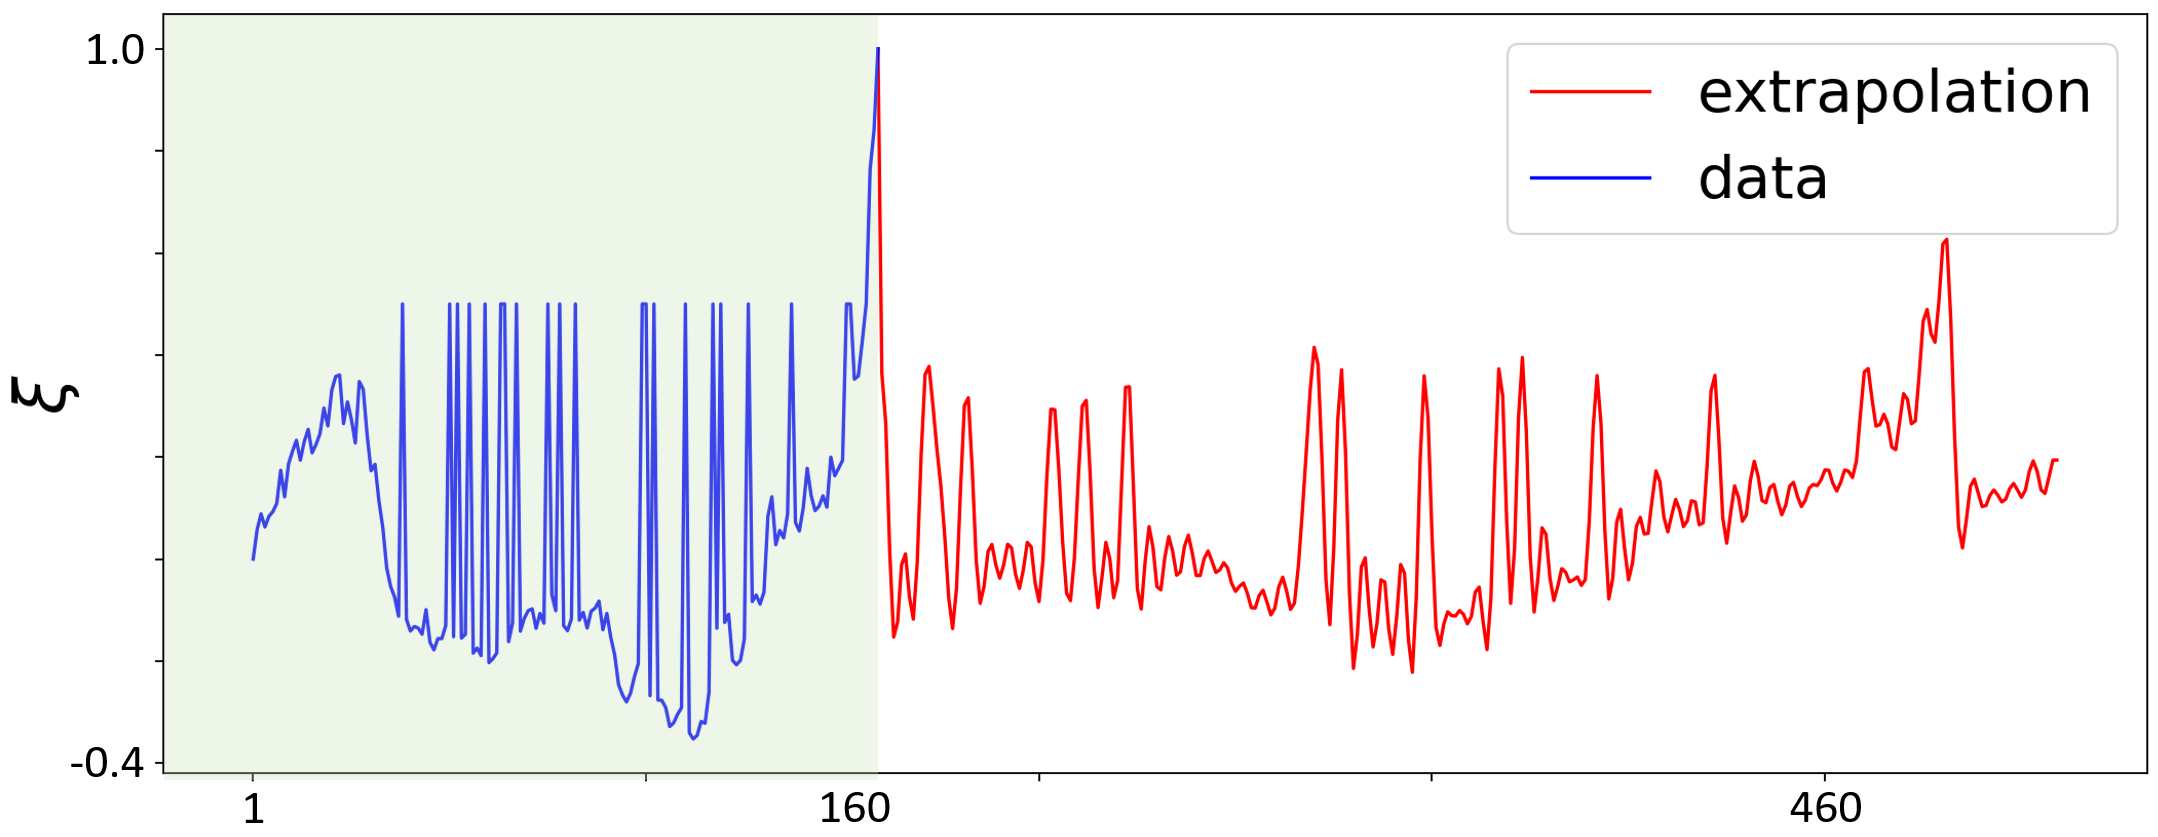
\includegraphics[width=1.0 \linewidth]{latex/images/rtextra/curve.png}
% % 
\includegraphics[width=1.0 \linewidth]{latex/images/rtextra/tet.png}
% \caption{Extrapolate head motion from input frames. For the left column: the first row is the sequence of input frames, the second row is the visualization of head motion for each input frame by applying the correspondence $[\mathbf{R},\mathbf{T}]$ to the reconstructed 3D face, and the third row is the parameterized motion $\xi_{1:\tau}$ for input frames. For the right column: the first row is the extrapolated frames of head motion visualization, and the second row is the extrapolated motion parameterization $\xi_{\tau+1:T}$.}
% \label{fig:rtextra}
% \end{figure}
 

% \subsection{The natural head motion extrapolation}
% \label{subsec:movement}

%To synthesize realistic talking-head videos, we introduce a head motion extrapolation method, which predicts the head movements $\hat{\mathbi{h}}_{\tau +1:T}$ based on the 3D landmarks $\mathbi{l}_{1:\tau}$ computed from ${\mathbi{y}}_{1:\tau}$. Thanks to the Lie Group framework for affine interpolation~\cite{bansal2019affine}, from two given affine transformations $\mathbb{T}_1$ and $\mathbb{T}_2$, an intermediate transformation can be represented as a $\mathbb{T}(\xi), \xi\in[0,1]$, such that $\mathbb{T}(0)=\mathbb{T}_1$ and $\mathbb{T}(1)=\mathbb{T}_2$. Specifically, for rigid transformation, the Lie group representation of the interpolated transformation between $[\mathbf{R},\mathbf{T}]_1$ and $[\mathbf{R},\mathbf{T}]_\tau$ at $\xi$, is given by:
%\begin{equation}
% \label{eqn:rtextra}
% [\mathbf{R},\mathbf{T}](\xi) = [\mathbf{R},\mathbf{T}]_1 \exp\left(\xi \log\left([\mathbf{R},\mathbf{T}]_1^{-1}[\mathbf{R},\mathbf{T}]_\tau\right)\right).
% \end{equation}
%Closed-form expressions of the exponential and log maps can be found in~\cite{bansal2019affine}.
%Therefore, $[\mathbf{R},\mathbf{T}]_{1:\tau}$ can be mapped to the parameter space $\xi_{1:\tau}=\{\xi_1,\xi_2,...,\xi_\tau\}$, such that $[\mathbf{R},\mathbf{T}](\xi_i)\approx [\mathbf{R},\mathbf{T}]_i$. Note that $\xi_1=0$, $\xi_\tau=1$ and $\xi_i (1<i<\tau)$ can be obtained by solving 
%$\underset{x}{\text{argmin}} \begin{Vmatrix}[\mathbf{R},\mathbf{T}](\xi_i) - [\mathbf{R},\mathbf{T}]_i\end{Vmatrix}_F$.
%We observed that the movement of a talking-head is bounded and has some periodic trend. Hence, we apply the Discrete Fourier Transformation on $\xi_i^\tau$ and choose the first $45$ harmonics to construct the Fourier series $\mathcal{F}(\cdot)$, such that $\mathcal{F}(i)\approx \xi_i, i\in[1,\tau]$. Then we can extrapolate $\xi_{\tau+1:T}$ by $\{\mathcal{F}(\tau+1),...,\mathcal{F}(T)\}$. Finally, applying  Eq.~\ref{eqn:rtextra} on $\xi_{\tau+1:T}$ will result to $[\hat{\mathbf{R}},\hat{\mathbf{T}]}_{\tau + 1:T}$.
%In Fig.~\ref{fig:rtextra}, we visualize the head motion by applying $[\mathbf{R},\mathbf{T}]_i$ to the reconstructed 3D face $\mathcal{M}$ and then rendering with the 3D Projector (see Sec.~\ref{subsec:3d_man}). The bottom curve in Fig.~\ref{fig:rtextra} is the parameter $\xi$ over time.


\section{Experiments}
\label{sec:experiments}
In this section, we conduct thoughtful experiments to demonstrate the effectiveness of the proposed architecture for video generation. 
%Sec. 4.1 explains datasets and implementation in detail. Sec. 4.2 shows our results along with other state-of-the-art methods. We show user studies and ablation study in Sec.4.3 and Sec. 4.4 respectively.

\subsection{Experimental Setup}
\label{subsec:exp_setup}

\noindent \textbf{Dataset} \quad We quantitatively and qualitatively evaluate our approach on three datasets with moving-talking-head videos: VoxCeleb2~\cite{Chung18b}, LRW~\cite{Chung16} and LRS3~\cite{Afouras18d}. The VoxCeleb2 contains over 1 million utterances for 6,112 celebrities, with large head motion. The LRW dataset consists of 500 different words spoken by hundreds of different speakers in the wild. Videos in LRS3~\cite{Afouras18d} contain more diverse and challenging head movements comparing to VoxCeleb2 and LRW.  We follow the same train-test split as in \cite{Chung18b,Chung16,Afouras18d}. 

\noindent \textbf{Implementation Details} \quad We follow the training procedure from \cite{wang2018fewshotvid2vid}. We adopt ADAM~\cite{KingmaB14} optimizer with $\text{lr} = 2 \times 10^{-4}$ and $(\beta_1,\beta_2) = (0.5,0.999)$. During training, we select $K = 1,8,32$ in our embedding network. The $\tau$ in all experiments is 64. The $\lambda_{\text{FM}} = 10$ and $\lambda_{\text{PCT}} = 1$ in Eq.~\ref{eq:loss}.  
%All experiments are conducted on an NVIDIA DGX-1 machine with 8 32GB V100 GPUs. 
  
 
%%%%%%%%%%%%%%%%%%%%%%%%%%
\begin{table}[t]
\scriptsize
    \centering
%   \begin{tabular*}{\linewidth}{  p{2.8cm}| p{0.9cm}  p{0.9cm} p{0.9cm} p{1.1cm} p{0.9cm} |p{0.9 cm} p{0.9cm} p{0.9cm} p{0.9cm}  }
\begin{tabular*}{\linewidth}{  l| c c c c c |c c c c}
      \toprule
      \hline
    %   \toprule
Method  & \multicolumn{9}{c}{Audio-driven}  \\ \hline
Dataset & \multicolumn{5}{c}{LRW} & \multicolumn{4}{c}{VoxCeleb2}  \\
    %   \midrule 
    % \hline
& {LMD$\downarrow$} & {CSIM$\uparrow$} & {FID$\downarrow$} & {Human$\downarrow$} & {WER$\downarrow$} & {LMD$\downarrow$} & {CSIM$\uparrow$} & {FID$\downarrow$} & {Human$\downarrow$}  \\

\hline
{Wiles et al., 2018~\cite{wiles2018x2face}} &  &    &   & &    &    &  \\
%  \hline
 {Chung et al., 2017~\cite{chung2017you}}&  &       &  & &   &    &     \\ %\hline

 {Chen et al., 2019~\cite{chen2019hierarchical}}  &   &   &   &  &   &   &  \\    %\hline
  {Song et al., 2019~\cite{ijcai2019-129}}  & \textbf{ } &   &   & & \textbf{ }   &  &  \\    %\hline
  {Vougioukas et al., 2019~\cite{vougioukas2019realistic}}  &   &   &   &  &     &        &  \\   

  {Zhou et al., 2019~\cite{zhou2019talking}}  &   &   &   &  &     &        &  \\   
    % \bottomrule
  { Ours (K=1)} &   & \textbf{  }& \textbf{   }&  &   &\textbf{      } &\textbf{      }\\ %\hline
    %   \bottomrule
  \end{tabular*}
  \caption{Quantitative results of different audio to video methods on LRW dataset and VoxCeleb2 dataset. Our model mentioned in this table are trained from scratch. We bold each leading score.}
    \label{tab:audio_tb}
\end{table}
%%%%%%%%%%%%%%%%%%%%%%%%%
%%%%%%%%%%%%%%%%%%%%%%%%%%

\begin{table}[t]
    \centering
    \scriptsize
    % \begin{center}
    \begin{tabular*}{0.98\linewidth}{  l | c c  c c| c c c c }
%   \begin{tabular*}{0.7\linewidth}{  p{2.8cm}| p{0.9cm} p{0.9cm} p{1.2cm} |p{1.2cm} p{0.9cm} p{0.9cm}}
      \toprule
      \hline
    %   \toprule
 Method & \multicolumn{8}{c}{Landmark-driven}   \\ \hline
Dataset & \multicolumn{4}{c}{LRS-TED} & \multicolumn{4}{c}{VoxCeleb2}  \\
    %   \midrule
&{{\scriptsize{CSIM}}$\uparrow$}& {{\scriptsize{SSIM}}$\uparrow$} & 
% {{\scriptsize{PSNR}}$\uparrow$}&
{{\scriptsize{FID}}$\downarrow$} & {{\scriptsize{Human}}$\uparrow$} &{{\scriptsize{CSIM}}$\uparrow$}  %{{\scriptsize{PSNR}}$\uparrow$}
& {{\scriptsize{CSIM}}$\uparrow$}&{{\scriptsize{FID}}$\downarrow$} & {{\scriptsize{Human}}$\uparrow$}   \\
%\hline  
{{\scriptsize{Wiles et al., 2018}~\cite{wiles2018x2face}}} &  &      &  &    &   &  \\ %\hline

{{\scriptsize{Chen et al., 2019}~\cite{chen2019hierarchical}}}&  &  & \textbf{  } &   &       &   \\   % \hline

% {{\scriptsize{Pix2pixHD}~\cite{wang2018high}}} & { 0.09 } &{ 0.56} &{ 42.7} & { 0.11 } &{ 0.52} &{ 43.9} \\ \hline
 {{\scriptsize{Zakharov et al., 2019~\cite{zakharov2019few} (K=1)}}} & {      } &{       } &{      } &     &     &         \\ %\hline
  {{\scriptsize{Wang et al., 2019~\cite{wang2018fewshotvid2vid} (K=1)}}} & { } &{ } &{ } & & &  & {} &{}\\ %\hline
 {{\scriptsize{Ours (K=1)} }}&\bf{   } & \bf{     } &{     } & \bf{      } & \bf{      } &\bf{      }  \\ 
%  \bottomrule
 \hline
 {{\scriptsize{Zakharov et al., 2019~\cite{zakharov2019few} (K=8)}}} & {      } &{       } &{      } &     &     &         \\ %\hline
  {{\scriptsize{Wang et al., 2019~\cite{wang2018fewshotvid2vid} (K=8)}}} & { } &{ } &{ } & & &  & {} &{} \\ %\hline
 {{\scriptsize{Ours(K=8)} }}&\bf{   } & \bf{     } &{     } & \bf{      } & \bf{      } &\bf{      }  \\
%   \bottomrule 
 \hline
 {{\scriptsize{Zakharov et al., 2019~\cite{zakharov2019few}(K=32)}}} & {      } &{       } &{      } &     &     &         \\ %\hline
  {{\scriptsize{Wang et al., 2019~\cite{wang2018fewshotvid2vid}(K=32)}}} & { } &{ } &{ } & & &  & {} &{}   \\ %\hline
 {{\scriptsize{Ours (K=32)} }}&\bf{   } & \bf{     } &{     } & \bf{      } & \bf{      } &\bf{      }  \\ 
    %   \bottomrule
  \end{tabular*}
%   \end{center}
  \caption{Quantitative results of different landmark to video methods on VoxCeleb1 dataset and VoxCeleb2 dataset. Our model mentioned in this table are trained from scratch. We bold each leading score. The number after each method denotes the $K$ frames of the target subject.}
    \label{tab:lmark_tb}
\end{table}
  
\subsection{Results and Analysis}
\label{subsec:quanti_res}
\noindent \textbf{Evaluation Metrics} \quad We use several criteria for quantitative evaluation. We use Fréchet Inception Distance (FID)~\cite{heusel2017gans}, mostly quantifying the fidelity of synthesized images, structured similarity (SSIM)~\cite{wang2004image}, commonly used to measure the low-level similarity between the real images and generated images. To evaluate the identity preserving ability, we use cosine similarity ({{CSIM}}) used in \cite{zakharov2019few}, which computes the cosine similarity between embedding vectors of the state-of-the-art face recognition network~\cite{deng2019arcface} for measuring identity mismatch. To evaluate whether the synthesized video contains accurate lip movements that correspond to the input condition, we adopt the evaluation matrix Landmarks Distance (LMD) proposed in~\cite{chen2018lip}. Additionally, we conduct user study to investigate the visual quality of the generated videos.{\lchen{lip reading}}


% \begin{figure}
% 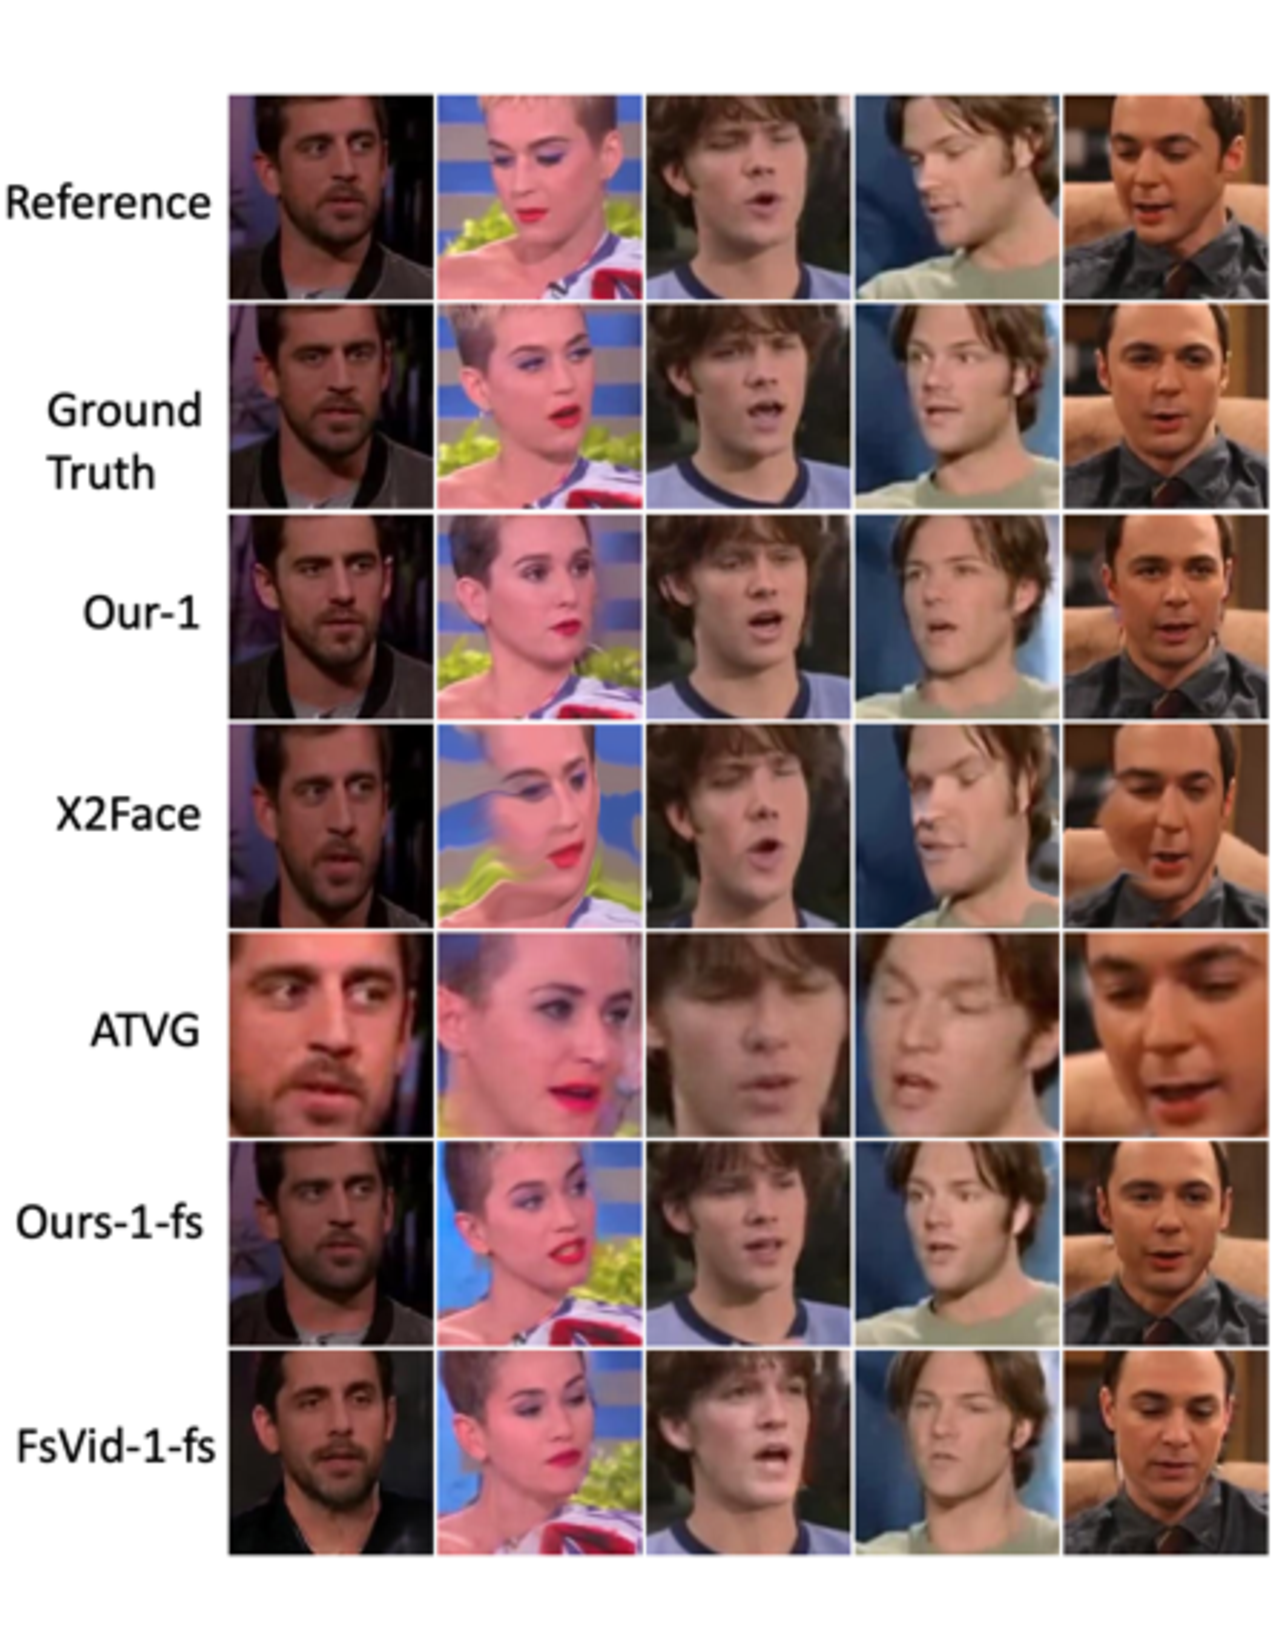
\includegraphics[width=0.95 \linewidth]{latex/images/compare1_reduce.pdf}
% \caption{The qualitative results of different landmark/image-driven methods on VoxCeleb2 testing set. The third to fifth rows are zero-shot results. The last two rows are one-shot results.}
% % \vspace{-6.5mm}
% \label{fig:compare1}
% \end{figure}


\noindent \textbf{Comparison with Audio-driven Methods.} \quad We first consider such a scenario that takes audio and one frame as inputs and synthesizes a talking face saying the speech, which has been explored in Chung et al.~\cite{chung2017you}, Wiles et al.~\cite{wiles2018x2face}, Chen et al.~\cite{chen2019hierarchical}, Song et al.~\cite{ijcai2019-129}, Vougioukas et al.~\cite{vougioukas2019realistic}, and Zhou et al.~\cite{zhou2019talking}. Comparing  with their methods, our method is able to generate vivid videos including controllable eye blinking, head movements, and natual facial expressions. Visual results Fig.XXXX . Quantitative results  ~\ref{tab:audio_tb}.

\noindent \textbf{Comparison with Visual-driven Methods.} \quad We also compare our approach with state-of-the-art landmark/image-driven generation methods: Zakharov et al.\cite{zakharov2019few}, Wiles et al.~\cite{wiles2018x2face}, and Wang et al.~\cite{wang2018fewshotvid2vid} on VoxCeleb2 and \lchen{other datasets} datasets. According to Tab.~\ref{tab:lmark_tb}, our approach achieves best performance in most of the evaluation matrices. It is worth to mention that our method outperforms other methods in terms of the CSIM score, which demonstrates the generalizability of our method. We choose different $K$ here to better understand our matching scheme. We can see that with larger $K$ value, the inception performance (FID and SSIM) improve dramatically. Note that we only select $K$ images from the first 64 frames, and  Zakharov et al., 2019~\cite{zakharov2019few} and  Wang et al., 2019~\cite{wang2018fewshotvid2vid} select $K$ images from the whole video sequence, which arguably gives other methods an advantage. Fig.XXXXX

\noindent \textbf{Comparison With Image Editing Methods.} 
% To further explore the upper-bound of our approach,
To further demonstrate the ability of our approach, we compare our method Suwajanakorn et al.~\cite{suwajanakorn2017synthesizing}. XXXXX


%%%%%%%%%%%%%%%%%%%%%%%%%%%%%%%%%%%%%%%
\begin{table}[t]
% \scriptsize
    \centering
  \begin{tabular*}{0.9\linewidth}{  p{4.2cm} | p{1.0cm} p{1.0cm} p{1.0cm} p{1.0cm} p{1.0cm} p{1.0cm} p{1.0cm}}
      \toprule
      \hline
    %   \midrule
Method & {CSIM$\uparrow$} &{PSNR$\uparrow$}  &{SSIM$\uparrow$}&{FID$\downarrow$} &{Human$\uparrow$}  \\ \hline
{w/o head motion } & \textbf{ } &  &\bf{}  \\ %\hline
{w/o 3D-Aware} & \textbf{ } &  &\bf{}  \\ %\hline
{w/o Hybrid-Attention} & \textbf{ } &  &\bf{}  \\ %\hline
{w/o None-linear comp.} & \textbf{ } &  &\bf{}  \\ %\hline
% {w/o warping} &     &     &     \\ %\hline
{w/o Motion Matcher}  &     &     &     \\ %\hline
{w/o temporal smoothing}  &     &     &     \\ %\hline
{with MFCC} & {     } & \bf{     } &  {     } \\ %\bottomrule
{Full, K=1} & \textbf{     } & \textbf{     } &  \textbf{     }\\ %\hline
{Full, K=8} & \textbf{     } & \textbf{     } &  \textbf{     }\\ %\hline
{Full, K=32} & \textbf{     } & \textbf{     } &  \textbf{     }\\ %\hline
    % \bottomrule
  \end{tabular*}
  \caption{Ablation studies on VoxCeleb2 dataset. Our model mentioned in this table are trained from scratch. We bold each leading score.}
    \label{tab:alation}
\end{table}
%%%%%%%%%%%%%%%%%%%%%%%%
\noindent \textbf{Ablation Studies} \quad We conduct thoughtful ablation experiments to study the contributions of each module we introduced in Sec.~\ref{sec:method} and Sec.~\ref{sec:3dgan}. The ablation studies are conducted on VoxCeleb2 dataset.
As shown in Tab.~\ref{tab:alation}, each component contributes to the full model. XXXXX
%We can find that the {Motion Matcher} is critical to our full model. We attribute it to the better ability of generating smooth transactions between adjacent frames. We also replace the dilation operation with warping to fix the $c_t$ caused by {Motion Matcher} and we can find that with warping, the performance drops. We attribute it to the poor ability of optic follow on complicated dynamics in head movements (e.g., head rotation). Also, we can find that with more reference images (larger $K$ value), our model achieves better performance. We attribute it to the lower $c_t$ since we have more choices to match the target frame. 

%\noindent \textbf{Qualitative Results} \quad We show our qualitative comparison in Fig.~\ref{fig:compare1} with other state-of-the-art methods. We can find that our approach can generate correct head motion and facial expressions, while preserving the appearance information. We show more audio-driven video results and interesting manipulations on head motion and facial expressions in \textit{Supplementary Material}   please refer to the video and images in the \textit{Supplementary Material}.

\section{Conclusion and Discussion}
In this paper, we propose a novel approach to model the head motion and facial expression explicitly, which can synthesize talking-head videos with rhythmic head motion of unseen subjects at the inference time. By leveraging the 3D manipulation, our model can generate talking-head videos with controllable head motion and facial expressions. Experimental results showed that our method performs favorably against the competing methods.
  

\clearpage

\bibliographystyle{splncs04}
\bibliography{review}
\end{document}
